% CMES / Tech Science Press formatted manuscript.
\documentclass[cmes,article,submit,moreauthors,pdftex]{Definitions/tsp}

%%%%Update on 30 November 2023%%%
\usepackage[normalem]{ulem} % For using the command \uuline{} in the \abstract 
\usepackage{amsfonts} % Use for some special math mark
%%\usepackage{pxfonts} % Use for some special math mark 
%\usepackage{wasysym} % Use for some special mark
%\usepackage{subfigure} % For some paper the use \subfigure
\usepackage{mathcomp} % For permille mark
\usepackage{CJKutf8} % For Chinese font
\usepackage{pifont} % For some special mark 
\usepackage{bm} % Forr math enviroment bold format
\usepackage{bbm} % For some math fancy characters
\graphicspath{{./Definitions/}} % Use for import path the figures paper used

\makeatletter
\def\T@n@@nc@d@ngM@cr@M@d{}
\def\LY@n@@nc@d@ngM@cr@M@d{}
\makeatother

\let\orignewcommand\newcommand  % Store the original \newcommand
\let\newcommand\providecommand  % Make \newcommand behave like \providecommand
\usepackage{verse}
\let\newcommand\orignewcommand  % Use the original `\newcommand` in future
\makeatletter
\renewcommand*{\theHpoemline}{\arabic{verse@envctr}.\arabic{poemline}} % Use the original definition from verse.sty
\makeatother

% Define a matrix envrioment
\newsavebox\foobox
\newcommand{\slantbox}[2][.2]{\mbox{%
        \sbox{\foobox}{#2}%
        \hskip\wd\foobox
        \pdfsave
        \pdfsetmatrix{1 0 #1 1}%
        \llap{\usebox{\foobox}}%
        \pdfrestore
}}

%\setlength{\fboxsep}{0cm}

% Define triangledown mark
\let\oldblacktriangledown\blacktriangledown

% Define \dagger using unicode
\renewcommand{\dagger}{\mathchar"2279}
\renewcommand{\ddagger}{\mathchar"227A}

% Define italic In, Max
\newcommand{\mmathit}[1]{
  \ifthenelse{\equal{#1}{\ln}}{\mathit{ln}}{
    \ifthenelse{\equal{#1}{\max}}{\mathit{max}}{\mathit{#1}}
  }
}
\makeatother
\robustify{\footnote}

\DeclareUnicodeCharacter{1E45}{\.{n}}
\DeclareUnicodeCharacter{1E41}{\.{m}}
\DeclareUnicodeCharacter{2003}{\quad}
%\DeclareUnicodeCharacter{0177}{\^{y}}
%\DeclareUnicodeCharacter{101}{\={a}}
\DeclareUnicodeCharacter{2009}{\thinspace}
\DeclareUnicodeCharacter{2002}{\enspace{}}
\DeclareUnicodeCharacter{2005}{\thinspace}
\DeclareUnicodeCharacter{0263}{\textipa{G}}
%\DeclareUnicodeCharacter{117}{\.{e}}
\DeclareUnicodeCharacter{A0}{~}
\DeclareUnicodeCharacter{2460}{\textcircled{\scriptsize{1}}}
\DeclareUnicodeCharacter{2461}{\textcircled{\scriptsize{2}}}
\DeclareUnicodeCharacter{2462}{\textcircled{\scriptsize{3}}}
\DeclareUnicodeCharacter{2463}{\textcircled{\scriptsize{4}}}
\DeclareUnicodeCharacter{2464}{\textcircled{\scriptsize{5}}}
\DeclareUnicodeCharacter{2465}{\textcircled{\scriptsize{6}}}
\DeclareUnicodeCharacter{2466}{\textcircled{\scriptsize{7}}}
\DeclareUnicodeCharacter{2467}{\textcircled{\scriptsize{8}}}
\DeclareUnicodeCharacter{2468}{\textcircled{\scriptsize{9}}}
\DeclareUnicodeCharacter{2070}{\textsuperscript{0}}
\DeclareUnicodeCharacter{2074}{\textsuperscript{4}}
\DeclareUnicodeCharacter{2075}{\textsuperscript{5}}
\DeclareUnicodeCharacter{2076}{\textsuperscript{6}}
\DeclareUnicodeCharacter{2077}{\textsuperscript{7}}
\DeclareUnicodeCharacter{2078}{\textsuperscript{8}}
\DeclareUnicodeCharacter{2079}{\textsuperscript{9}}
\DeclareUnicodeCharacter{02C2}{<}
\DeclareUnicodeCharacter{2033}{\relax\ifmmode '' \else $''$\fi}
\DeclareUnicodeCharacter{2034}{\relax\ifmmode ''' \else $'''$\fi}
\DeclareUnicodeCharacter{2026}{\relax\ifmmode … \else $\ldots$\fi}
\DeclareUnicodeCharacter{0229}{\c{e}}
\DeclareUnicodeCharacter{016F}{\r{u}}
%\DeclareUnicodeCharacter{0218}{\cb{S}}
%\DeclareUnicodeCharacter{0219}{\cb{s}}
%\DeclareUnicodeCharacter{021B}{\cb{t}}
\DeclareUnicodeCharacter{127}{\relax\ifmmode\rm\hbar\else $\rm\hbar$\fi}
\DeclareUnicodeCharacter{3AC}{\relax\ifmmode\acute{\alpha}\else $\acute{\alpha}$\fi}
\DeclareUnicodeCharacter{3AD}{\relax\ifmmode\acute{\varepsilon}\else $\acute{\varepsilon}$\fi}
\DeclareUnicodeCharacter{3AE}{\relax\ifmmode\acute{\eta}\else $\acute{\eta}$\fi}
\DeclareUnicodeCharacter{3AF}{\relax\ifmmode\acute{\iota}\else $\acute{\iota}$\fi}
\DeclareUnicodeCharacter{3CC}{\relax\ifmmode\acute{o}\else $\acute{o}$\fi}
\DeclareUnicodeCharacter{3CD}{\relax\ifmmode\acute{\upsilon}\else $\acute{\upsilon}$\fi}
\DeclareUnicodeCharacter{3CE}{\relax\ifmmode\acute{\omega}\else $\acute{\omega}$\fi}
\DeclareUnicodeCharacter{391}{A}
\DeclareUnicodeCharacter{392}{B}
\DeclareUnicodeCharacter{395}{E}
\DeclareUnicodeCharacter{396}{Z}
\DeclareUnicodeCharacter{397}{H}
\DeclareUnicodeCharacter{399}{I}
\DeclareUnicodeCharacter{39A}{K}
\DeclareUnicodeCharacter{39C}{M}
\DeclareUnicodeCharacter{39D}{N}
\DeclareUnicodeCharacter{39F}{O}
\DeclareUnicodeCharacter{3A1}{P}
\DeclareUnicodeCharacter{3A4}{T}
\DeclareUnicodeCharacter{3A7}{X}

\DeclareUnicodeCharacter{27E6}{\relax\ifmmode \llbracket \else $\llbracket$\fi}
\DeclareUnicodeCharacter{27E7}{\relax\ifmmode \rrbracket \else $\rrbracket$\fi}
\DeclareUnicodeCharacter{00B5}{\relax\ifmmode \mu{} \else $\mu$\fi}
\DeclareUnicodeCharacter{1D434}{\relax\ifmmode A \else $A$\fi}
\DeclareUnicodeCharacter{1D435}{\relax\ifmmode B \else $B$\fi}
\DeclareUnicodeCharacter{1D436}{\relax\ifmmode C \else $C$\fi}
\DeclareUnicodeCharacter{1D437}{\relax\ifmmode D \else $D$\fi}
\DeclareUnicodeCharacter{1D438}{\relax\ifmmode E \else $E$\fi}
\DeclareUnicodeCharacter{1D439}{\relax\ifmmode F \else $F$\fi}
\DeclareUnicodeCharacter{1D43A}{\relax\ifmmode G \else $G$\fi}
\DeclareUnicodeCharacter{1D43B}{\relax\ifmmode H \else $H$\fi}
\DeclareUnicodeCharacter{1D43C}{\relax\ifmmode I \else $I$\fi}
\DeclareUnicodeCharacter{1D43D}{\relax\ifmmode J \else $J$\fi}
\DeclareUnicodeCharacter{1D43E}{\relax\ifmmode K \else $K$\fi}
\DeclareUnicodeCharacter{1D43F}{\relax\ifmmode L \else $L$\fi}
\DeclareUnicodeCharacter{1D440}{\relax\ifmmode M \else $M$\fi}
\DeclareUnicodeCharacter{1D441}{\relax\ifmmode N \else $N$\fi}
\DeclareUnicodeCharacter{1D442}{\relax\ifmmode O \else $O$\fi}
\DeclareUnicodeCharacter{1D443}{\relax\ifmmode P \else $P$\fi}
\DeclareUnicodeCharacter{1D444}{\relax\ifmmode Q \else $Q$\fi}
\DeclareUnicodeCharacter{1D445}{\relax\ifmmode R \else $R$\fi}
\DeclareUnicodeCharacter{1D446}{\relax\ifmmode S \else $S$\fi}
\DeclareUnicodeCharacter{1D447}{\relax\ifmmode T \else $T$\fi}
\DeclareUnicodeCharacter{1D448}{\relax\ifmmode U \else $U$\fi}
\DeclareUnicodeCharacter{1D449}{\relax\ifmmode V \else $V$\fi}
\DeclareUnicodeCharacter{1D44A}{\relax\ifmmode W \else $W$\fi}
\DeclareUnicodeCharacter{1D44B}{\relax\ifmmode X \else $X$\fi}
\DeclareUnicodeCharacter{1D44C}{\relax\ifmmode Y \else $Y$\fi}
\DeclareUnicodeCharacter{1D44D}{\relax\ifmmode Z \else $Z$\fi}
\DeclareUnicodeCharacter{1D44E}{\relax\ifmmode a \else $a$\fi}
\DeclareUnicodeCharacter{1D44F}{\relax\ifmmode b \else $b$\fi}
\DeclareUnicodeCharacter{1D450}{\relax\ifmmode c \else $c$\fi}
\DeclareUnicodeCharacter{1D451}{\relax\ifmmode d \else $d$\fi}
\DeclareUnicodeCharacter{1D452}{\relax\ifmmode e \else $e$\fi}
\DeclareUnicodeCharacter{1D453}{\relax\ifmmode f \else $f$\fi}
\DeclareUnicodeCharacter{1D454}{\relax\ifmmode g \else $g$\fi}
\DeclareUnicodeCharacter{1D456}{\relax\ifmmode i \else $i$\fi}
\DeclareUnicodeCharacter{1D457}{\relax\ifmmode j \else $j$\fi}
\DeclareUnicodeCharacter{1D458}{\relax\ifmmode k \else $k$\fi}
\DeclareUnicodeCharacter{1D459}{\relax\ifmmode l \else $l$\fi}
\DeclareUnicodeCharacter{1D45A}{\relax\ifmmode m \else $m$\fi}
\DeclareUnicodeCharacter{1D45B}{\relax\ifmmode n \else $n$\fi}
\DeclareUnicodeCharacter{1D45C}{\relax\ifmmode o \else $o$\fi}
\DeclareUnicodeCharacter{1D45D}{\relax\ifmmode p \else $p$\fi}
\DeclareUnicodeCharacter{1D45E}{\relax\ifmmode q \else $q$\fi}
\DeclareUnicodeCharacter{1D45F}{\relax\ifmmode r \else $r$\fi}
\DeclareUnicodeCharacter{1D460}{\relax\ifmmode s \else $s$\fi}
\DeclareUnicodeCharacter{1D461}{\relax\ifmmode t \else $t$\fi}
\DeclareUnicodeCharacter{1D462}{\relax\ifmmode u \else $u$\fi}
\DeclareUnicodeCharacter{1D463}{\relax\ifmmode v \else $v$\fi}
\DeclareUnicodeCharacter{1D464}{\relax\ifmmode w \else $w$\fi}
\DeclareUnicodeCharacter{1D465}{\relax\ifmmode x \else $x$\fi}
\DeclareUnicodeCharacter{1D466}{\relax\ifmmode y \else $y$\fi}
\DeclareUnicodeCharacter{1D467}{\relax\ifmmode z \else $z$\fi}

\DeclareUnicodeCharacter{1E67}{\.{\v s}}
\DeclareUnicodeCharacter{1E11}{\relax\ifmmode \c{d} \else $\c{d}$\fi}
\DeclareUnicodeCharacter{1ECB}{\relax\ifmmode \d{i} \else $\d{i}$\fi}
\DeclareUnicodeCharacter{1D8D}{\relax\ifmmode \textlhookx \else $\textlhookx$\fi}
\DeclareUnicodeCharacter{104}{\relax\ifmmode \k{A} \else $\k{A}$\fi}
\DeclareUnicodeCharacter{211E}{\relax\ifmmode \textrecipe \else $\textrecipe$\fi}
\DeclareUnicodeCharacter{29D}{\relax\ifmmode \textctj \else $\textctj$\fi}

\DeclareUnicodeCharacter{1E2E}{\'{\"I}}
\DeclareUnicodeCharacter{23F}{\textrts}

\DeclareUnicodeCharacter{2C73}{\varw}

\DeclareUnicodeCharacter{2127}{\mho}

\DeclareUnicodeCharacter{28C}{\textturnv}
\DeclareUnicodeCharacter{252}{\textturnscripta}
\DeclareUnicodeCharacter{259}{\schwa}
\DeclareUnicodeCharacter{25B}{\m{e}}
\DeclareUnicodeCharacter{266}{\m{h}}
\DeclareUnicodeCharacter{127}{\B{h}}
\DeclareUnicodeCharacter{27E}{\textfishhookr}
\DeclareUnicodeCharacter{281}{\textinvscr}



\graphicspath{{figures/}{figures/validation/}{Definitions/}}
\usepackage{verbatim}
\SetMathAlphabet{\mathcal}{normal}{OMS}{cmsy}{m}{n}
\SetMathAlphabet{\mathcal}{bold}{OMS}{cmsy}{b}{n}
\setlength{\headheight}{38.22325pt}

\continuouspages{}
\firstpage{1}
\makeatletter
\setcounter{page}{\@firstpage}
\makeatother
\pubvolume{0}
\issuenum{0}
\elocationid{0}
\articlenumber{0}
\pubyear{2026}
\copyrightyear{2026}
\datereceived{Day Month Year}
\dateaccepted{Day Month Year}
\dateonlinefirst{}
\datepublished{Day Month Year}

\Title{Simulation-Based Bayesian Computational Decision Model for Risk--Resilience Structural Maintenance under Epistemic Uncertainty}
\TitleCitation{Simulation-Based Bayesian Computational Decision Model for Risk--Resilience Structural Maintenance under Epistemic Uncertainty}

\Author{Luis Rojas-Valdivia\textsuperscript{1} and Jose Garcia\textsuperscript{2,*}}
\AuthorNames{Luis Rojas-Valdivia and Jose Garcia}
\AuthorCitation{Rojas-Valdivia, L.; Garcia, J.}

\address{%
\textsuperscript{1}Doctorado en Industria Inteligente, Pontificia Universidad Catolica de Valparaiso, Valparaiso, Chile\\
\textsuperscript{2}Escuela de Ingenieria de Construccion y Transporte, Pontificia Universidad Catolica de Valparaiso, Valparaiso, Chile}
\corres{Corresponding Author: Jose Garcia. Email: to be provided}

\abstract{Engineering maintenance decisions often require uncertain evidence, simulated structural response, consequence descriptors, recovery effects, and resource constraints to be converted into a reproducible computational policy. This paper develops the Dynamic Structural Maintenance Prioritization (DSMP) model, a Bayesian risk--resilience decision model for structural maintenance prioritization under epistemic uncertainty. Count evidence is updated with a Gamma--Poisson model, consequences are decomposed into safety, operational, and environmental components, recovery impact is represented through a normalized recovery-time penalty, and epistemic uncertainty is made auditable through posterior variance, data-quality penalties, and model--data discrepancy. The resulting computational operator is embedded in value-of-information routing and in budget- and capacity-constrained action selection. The evaluation uses a simulation-based ground-truth protocol in which a degradation and limit-state simulator generates true failure probabilities, consequences, recovery exposure, and imperfect inspection evidence. Competing policies are compared using independent metrics, including Brier score, expected calibration error, regret relative to a ground-truth oracle, risk reduction per cost, downtime reduction, rank correlation, top-k capture, rank-reversal frequency, paired regret tests, and NSGA-II multiobjective Pareto feasibility. In the full validation run with 300 assets, 50 random seeds, and 256 Monte Carlo paths per asset, the uncalibrated Gamma--Poisson predictive probability was poorly calibrated against the simulated physical truth. Cross-fitted Platt recalibration reduced the median Brier score from 0.492 to 0.171 and the median expected calibration error from 0.565 to 0.033. At the selected budget level, the cost-aware DSMP direct policy using Platt-recalibrated probabilities achieved lower median regret than probability--consequence, greedy cost--risk, robust TOPSIS, and static RCM-like baselines, while policies using the simulated true failure probability remained better, as expected. Reference-based normalization avoided the rank reversals observed under portfolio min--max scaling. The study provides a transparent computational workflow for linking Bayesian updating, model-mismatch assessment, uncertainty-aware decision scoring, and constrained maintenance optimization.}

\keyword{computational decision modeling; Bayesian updating; simulation-based validation; maintenance optimization; value of information; epistemic uncertainty; resilience; structural reliability}

\begin{document}

\section{Introduction}

Computational maintenance planning for engineering systems involves more than ranking visible defects or applying fixed inspection intervals. A maintenance action changes the future state of the structure, the availability of information, the allocation of crews and budget, and the ability of the system to recover after disruption. The computational problem is to transform heterogeneous and uncertain evidence into a reproducible action policy while preserving the assumptions behind probability, consequence, recovery, uncertainty, and resource feasibility. In structural applications, this problem intersects reliability analysis, deterioration modeling, simulation, quality assurance, engineering judgement, decision analysis, and risk management \cite{rackwitz2001,frangopol2004,derkiureghian2009}.

Classical reliability-centered maintenance and risk-based inspection provide a useful foundation because they connect failure modes, failure probability, and consequence. However, structural systems often require a broader decision view. A component with moderate probability of failure may become critical if its loss delays recovery, blocks access, amplifies cascading effects, or is poorly observed. Conversely, a severe-looking defect may be less urgent if redundancy and accessibility limit its system-level effect. The practical question is therefore not only ``which component is most damaged?'' but also ``which intervention best reduces future risk and recovery burden under incomplete evidence and limited resources?'' \cite{bruneau2003,cimellaro2010,thons2018}.

This paper develops the Dynamic Structural Maintenance Prioritization (DSMP) index for that decision layer. DSMP combines Bayesian failure probability, consequence, recovery-time exposure, and epistemic uncertainty into a normalized maintenance priority. It is designed to remain auditable: each term can be traced to a probability model, an engineering consequence model, a recovery estimate, or a data-quality and model-discrepancy descriptor. The index is then connected to value-of-information (VoI) routing and resource-constrained action selection, so that uncertain assets can be directed toward inspection or monitoring rather than immediate repair when additional information is expected to be valuable.

The methodological design addresses a common validation difficulty in priority scoring: a score can appear useful when it is evaluated only on variables already embedded in its definition. The simulation-based ground-truth protocol reduces this circularity by generating true failure probabilities and true preventable losses through a separate degradation and limit-state process. The maintenance policies are then evaluated by independent quantities such as calibration error, regret relative to a ground-truth oracle, risk reduction per unit cost, and simulated downtime reduction. The synthetic evidence is used to make the evaluation target observable and independent from the proposed score.

The article contributes:
\begin{enumerate}[leftmargin=*]
    \item a Bayesian computational decision operator that generalizes probability--consequence risk by adding recovery and epistemic terms;
    \item a simulation-based ground-truth generator that combines degradation, limit-state failure, imperfect count evidence, and oracle decision metrics;
    \item a recalibration and model-mismatch assessment layer for comparing count-based predictive probabilities with simulated physical truth;
    \item a constrained action-selection workflow with VoI routing, reference-based normalization, graph-aware recovery adjustment, and NSGA-II Pareto feasibility checks;
    \item a structural-maintenance interpretation that shows how simulation, inspection, monitoring, and digital-twin outputs can feed the same decision model.
\end{enumerate}
Together, these elements establish a reproducible computational decision-analysis layer that can be challenged against controlled ground-truth experiments and then coupled to historical inspection, monitoring, or structural simulation records.

\section{Computational Modeling Background and Positioning}

\subsection{From reliability-centered maintenance to risk-based structural planning}

Reliability-centered maintenance (RCM) remains a useful starting point because it connects required functions, functional failures, failure modes, local effects, system effects, and technically justified preventive tasks. Its weakness for structural systems is not conceptual, but operational: the resulting prioritization can become semi-static when deterioration, inspection evidence, load exposure, consequence, and operating context are not updated over time \cite{dekker1996,wang2002,garg2006,ahmad2012}. This limitation is relevant for bridges and constructed facilities, where the priority of an intervention may change after new inspection evidence, traffic or operational changes, deterioration acceleration, load redistribution, or access constraints \cite{frangopol2004,frangopol2016}.

Risk-based inspection and maintenance address part of this problem by allocating effort according to probability and consequence. In structural reliability language, the event of interest is a failure or serviceability exceedance defined through a limit state $g_i(t)=R_i(t)-S_i(t)$, where $R_i(t)$ is resistance and $S_i(t)$ is demand. Bayesian updating then provides a principled mechanism for combining prior information with inspection, monitoring, and model evidence \cite{rackwitz2001,derkiureghian2009,beck1998,kennedy2001}. However, the standard probability--consequence product remains incomplete when recovery capacity, system coupling, information quality, and epistemic uncertainty are treated only qualitatively or outside the ranking model \cite{straub2005,sorensen2009,thons2018}.

Life-cycle structural reliability and inspection-planning research has developed strong methods for deteriorating structures, bridge systems, and infrastructure maintenance under uncertainty \cite{frangopol2004,estes2001,memarzadeh2016,papakonstantinou2014a,papakonstantinou2014b}. These works show that maintenance planning is inherently sequential and uncertain. At the same time, many practical prioritization tools still rely on a simpler decision surface: condition severity, failure probability, consequence class, or a weighted criticality matrix. The gap addressed here is not the absence of reliability theory, but the lack of a compact and auditable operator that keeps probability, consequence, recovery, uncertainty, graph position, information value, and resource feasibility visible in one constrained decision layer.

\subsection{Monitoring, digital twins, resilience, and interdependence}

Predictive maintenance and structural health monitoring have expanded the evidence base by introducing sensor data, inspection histories, diagnostic features, and prognostic indicators into asset management workflows \cite{jardine2006,worden2004,carden2004,farrar2007,brownjohn2007}. Digital-twin research extends this trajectory by synchronizing physical state, simulation, monitoring, and operational context \cite{tao2018,tao2019,fuller2020,rasheed2020,boje2020,lu2020}. For structural safety, however, state estimation is only one part of the problem. The estimated state must still be transformed into a defensible action: inspect, monitor, repair, reinforce, replace, or defer under limited budget, crews, access windows, and risk tolerance.

Resilience analysis adds another missing dimension. A structural component may become critical because its loss delays recovery, blocks access, amplifies cascading effects, or degrades system function for a long period, even when its local failure probability is moderate \cite{bruneau2003,cimellaro2010,francis2014,hosseini2016}. Interdependent infrastructure research further shows that local failures can propagate through functional, logistical, or network dependencies \cite{rinaldi2001,ouyang2014,buldyrev2010,gao2012,newman2003}. These ideas motivate the graph-aware recovery and cascade-susceptibility terms used in this manuscript as interpretable computational descriptors of system exposure.

Decision analysis and value-of-information theory provide the final piece of the state of the art. When evidence is poor or conflicting, the best immediate action may be inspection or monitoring rather than physical intervention. VoI-based planning has a strong basis in structural integrity management and is distinct from one-step repair benefit: acquiring information may increase immediate regret while improving the evidence state for subsequent actions \cite{thons2018,memarzadeh2016,papakonstantinou2014a,andriotis2019}. This distinction is central to the present results, where the DSMP direct and DSMP + VoI policies are reported separately.

\subsection{Computational decision modeling under uncertainty}

The computational literature on engineering decision support provides the modeling context for the proposed framework. Bayesian decision analysis connects uncertain evidence with decision variables; stochastic simulation provides controlled ground truth when field outcomes are unavailable or sparse; Monte Carlo evaluation quantifies the effect of probabilistic assumptions; and recalibration methods expose model mismatch between a predictive probability and an observed or simulated event process \cite{beck1998,kennedy2001,helton2006,saltelli2010}. These elements are especially relevant when the available evidence stream is informative but not identical to the physical limit-state process that controls failure.

Optimization and multi-criteria decision analysis provide complementary views of the action-selection problem. Weighted value models and outranking methods make trade-offs among risk, cost, uncertainty, and recovery explicit, while evolutionary multiobjective algorithms explore nondominated policies when objectives cannot be collapsed into a single scalar preference \cite{saaty2008,brans1985,roy1991,deb2002,coello2004,blank2020pymoo}. For maintenance planning, the computational challenge is to connect these methods to an engineering state description: degradation, failure probability, consequence, recovery burden, information quality, and feasible actions.

This paper brings these components into a single executable workflow. Bayesian updating produces predictive failure probabilities, the limit-state simulator supplies independent truth for validation, recalibration quantifies model mismatch, the DSMP score maps evidence to a decision attribute, and constrained policies translate the score into feasible actions. The resulting workflow is intended to be inspected algorithmically as well as interpreted physically.

\subsection{Research gap and positioning of the proposed operator}

The reviewed literature supports four requirements for a CMES-oriented contribution in this application domain. First, the model should remain compatible with structural reliability and limit-state thinking. Second, it should not collapse consequence, recovery, and uncertainty into an opaque condition score. Third, it should distinguish direct intervention from information acquisition. Fourth, it should be evaluated against quantities that are not already embedded in the score. The present paper responds to these requirements by formulating a Bayesian risk--resilience computational operator and then testing it against a synthetic ground-truth limit-state simulator.

Table~\ref{tab:paradigm-gap} summarizes this positioning qualitatively and makes explicit which limitation of each paradigm motivates the proposed decision operator.

\begin{table}[H]
\centering
\scriptsize
\caption{Qualitative positioning of the proposed operator relative to established engineering maintenance and computational-decision paradigms.}
\label{tab:paradigm-gap}
\begin{tabular*}{\textwidth}{@{\extracolsep{\fill}}>{\raggedright\arraybackslash}p{0.20\textwidth}>{\raggedright\arraybackslash}p{0.33\textwidth}>{\raggedright\arraybackslash}p{0.38\textwidth}}
\toprule
Paradigm & Main strength & Limitation addressed by the proposed operator \\
\midrule
RCM & Failure-mode and functional logic & Prioritization can remain semi-static when probability, evidence, and operating context are not updated. \\
RBI & Probability--consequence prioritization & Recovery capacity, observability, and epistemic uncertainty are often external to the ranking. \\
SHM/PdM & Condition inference and monitoring evidence & Health indicators are often component-centered and not directly tied to constrained action selection. \\
MCDA/optimization & Explicit computational trade-offs & Criteria, calibration, simulated truth, and feasible maintenance actions are often handled in separate layers. \\
Digital twins & State synchronization and what-if analysis & A transparent decision layer is still needed to convert state estimates into feasible maintenance actions. \\
\bottomrule
\end{tabular*}
\end{table}

The proposed operator can also be read at two decision levels. At the portfolio level, aggregated scores indicate whether the maintenance regime is dominated by failure risk, recovery vulnerability, poor observability, or resource scarcity. At the asset level, the same components rank feasible local actions such as inspection, monitoring, repair, reinforcement, replacement, or deferral. This two-level reading keeps strategic maintenance planning separate from local action assignment while preserving a common set of auditable decision variables.

The framework consumes outputs that finite-element analysis, structural health monitoring, digital twins, or learning-based prognostic models may provide: updated failure probability, degradation state, consequence descriptors, recovery estimates, graph dependence, and uncertainty descriptors. These upstream models supply evidence; the proposed contribution is the computational decision layer that organizes the evidence into an auditable and constrained maintenance plan.

Figure~\ref{fig:decision-architecture} summarizes this data-to-decision architecture. Inspection, monitoring, structural analysis, and operational information enter as evidence streams. The Bayesian update, consequence model, recovery model, epistemic audit, and graph layer then produce decision variables that can be inspected before an action is selected. This architecture connects the mathematical index with a reproducible computational workflow for engineering maintenance decisions.

\begin{figure}[H]
\centering
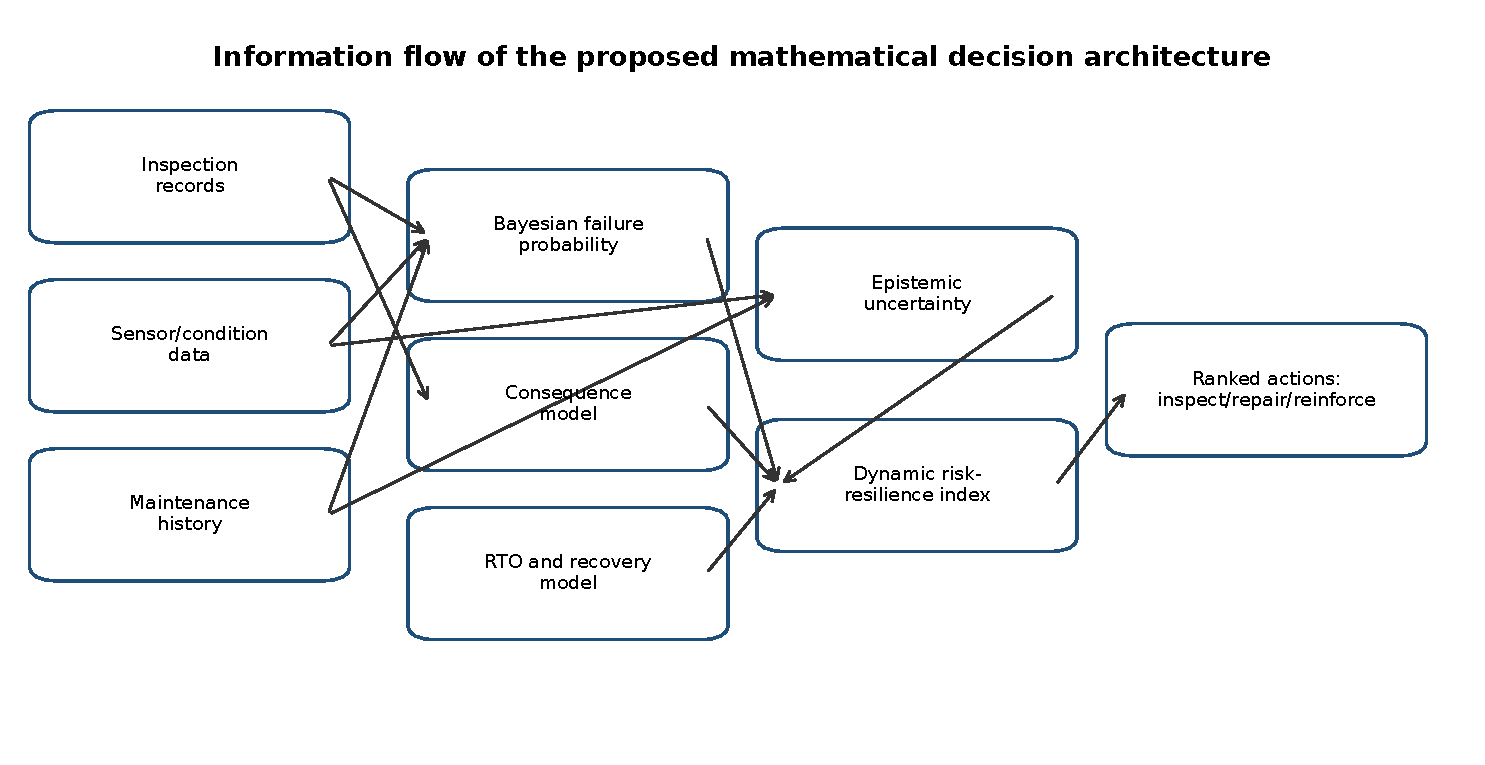
\includegraphics[width=0.88\textwidth]{fig02_decision_architecture.pdf}
\caption{Decision architecture linking structural evidence, Bayesian updating, consequence and recovery modeling, epistemic uncertainty, graph dependence, and constrained maintenance action selection.}
\label{fig:decision-architecture}
\end{figure}

The validation portfolio is synthetically generated so that physical truth, oracle action benefit, and calibration targets are observable. This makes the experiment a controlled computational benchmark: each policy is evaluated against quantities produced by the degradation and limit-state simulator rather than by its own score components. The same data interfaces can ingest retrospective inspection records, monitoring streams, finite-element outputs, or digital-twin state estimates when those records are available.

\section{Bayesian risk--resilience maintenance operator}

\subsection{Bayesian failure probability}

Let $i\in\mathcal{S}$ index a structural asset and let $D_t$ denote evidence available up to decision time $t$. The updated failure probability over a horizon $\tau$ is
\begin{equation}
P_i(t,\tau)=P(F_i\mid D_t,\theta_i),
\end{equation}
where $\theta_i$ denotes model and degradation parameters. For count-type evidence, the implementation uses a Gamma--Poisson model. If
\begin{equation}
\lambda_i \sim \mathrm{Gamma}(\alpha_0,\beta_0),
\qquad n_i(t)\mid \lambda_i \sim \mathrm{Poisson}(\lambda_i T_i),
\end{equation}
with $\beta$ expressed as a rate parameter, the posterior is
\begin{equation}
\lambda_i\mid D_t \sim \mathrm{Gamma}(\alpha_0+n_i(t),\beta_0+T_i).
\end{equation}
The plug-in estimate is
\begin{equation}
P_i^{\mathrm{plug}}(\tau)=1-\exp[-E(\lambda_i\mid D_t)\tau],
\end{equation}
and the exact posterior predictive probability is
\begin{equation}
P_i^{\mathrm{pred}}(\tau)=1-\left(\frac{\beta_i}{\beta_i+\tau}\right)^{\alpha_i},
\qquad \alpha_i=\alpha_0+n_i(t),\quad \beta_i=\beta_0+T_i.
\label{eq:predictive}
\end{equation}
The implementation stores both values. The plug-in probability is retained for interpretability, while the predictive probability is used in the validation layer because it follows directly from posterior marginalization.

\begin{figure}[H]
\centering
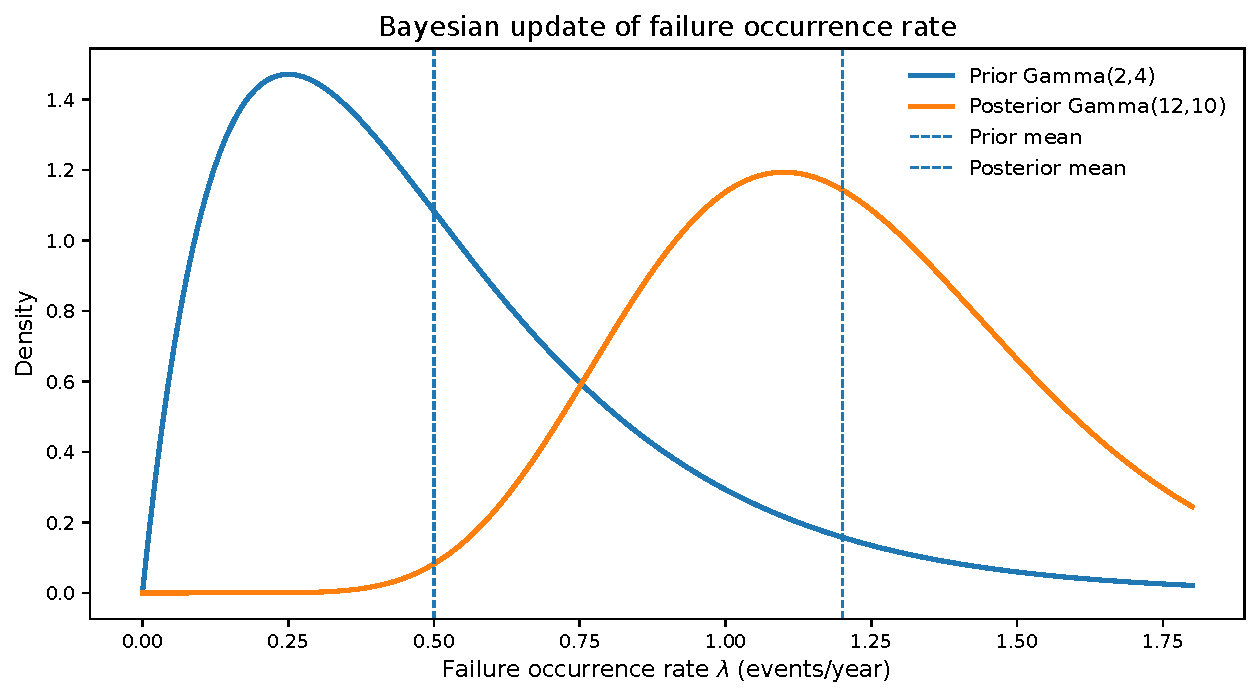
\includegraphics[width=0.68\textwidth]{fig05_bayesian_update_gamma_poisson.pdf}
\caption{Gamma--Poisson evidence update used for count-type observations. The posterior distribution supplies both a transparent rate estimate and the posterior predictive probability used in the validation protocol.}
\label{fig:gamma-poisson}
\end{figure}

\subsection{Consequence, recovery, and uncertainty}

The consequence term is decomposed into safety, operational, and environmental components:
\begin{equation}
\widetilde{C}_i=
\omega_s C_i^{safety}+\omega_p C_i^{operational}+\omega_e C_i^{environment},
\qquad \omega_s+\omega_p+\omega_e=1.
\end{equation}
The recovery term is represented by a normalized recovery-time impact $\widetilde{RTO}_i\in[0,1]$. The reference-based normalization used in the validation protocol is
\begin{equation}
\widetilde{y}_i^{ref}=
\mathrm{clip}\left(\frac{y_i-y_-^{ref}}{y_+^{ref}-y_-^{ref}},0,1\right),
\label{eq:reference-normalization}
\end{equation}
which avoids changing the score of existing assets when an extreme asset is inserted into the portfolio.

The epistemic term is made auditable by separating posterior variance, data quality, and model discrepancy:
\begin{equation}
\widetilde{U}_i(t)=
a_1 \widetilde{\mathrm{Var}}[P_i(t)] + a_2 Q_i(t) + a_3 M_i(t),
\qquad a_1+a_2+a_3=1.
\end{equation}
The data-quality penalty is computed from observable components \cite{derkiureghian2009,helton2006,saltelli2010}:
\begin{align}
q_i^{comp} &= \frac{n_i^{available}}{n_i^{required}}, &
q_i^{rec} &= \exp\left(-\frac{\Delta t_i^{last}}{T_{ref}}\right),\\
q_i^{sensor} &= 1-p_i^{missing}, &
q_i^{cons} &= 1-\frac{n_i^{conflict}}{n_i^{records}+\epsilon}.
\end{align}
Then
\begin{equation}
Q_i(t)=1-\left(w_{comp}q_i^{comp}+w_{rec}q_i^{rec}
+w_{sensor}q_i^{sensor}+w_{cons}q_i^{cons}\right).
\end{equation}
The model-discrepancy penalty is
\begin{equation}
M_i(t)=\mathrm{clip}\left(\frac{|\widehat{m}_i^{phys}(t)-\widehat{m}_i^{data}(t)|}{m_{ref}},0,1\right).
\end{equation}
This decomposition separates distinct decision roles. The product $P_i(t)\widetilde{C}_i$ carries the failure-conditioned risk contribution. The term $\widetilde{U}_i(t)$ describes lack of evidence, data conflict, or model--data discrepancy, and is therefore an audit variable rather than a second failure probability. The VoI gate uses this audit variable to identify cases where additional information may be worth acquiring. A positive weight $\eta$ then represents a conservative preference for acting on poorly evidenced assets when the decision maker wants uncertainty itself to affect priority. Keeping these roles explicit reduces the risk of double counting: physical failure likelihood enters through $P_i(t)$, while epistemic incompleteness enters through $\widetilde{U}_i(t)$ and the information-routing rule.

\subsection{Priority index and value-of-information routing}

The dynamic risk--resilience score is
\begin{equation}
\widetilde{R}_i(t)=
\alpha P_i(t)\widetilde{C}_i + \rho \widetilde{RTO}_i + \eta \widetilde{U}_i(t),
\qquad \alpha+\rho+\eta=1.
\label{eq:score}
\end{equation}

Equation~\eqref{eq:score} can be read as an additive value model over three normalized attributes: expected failure consequence, recovery exposure, and epistemic incompleteness. This interpretation is appropriate when the decision maker accepts preferential independence among these attributes over the local range of maintenance alternatives. The weights $(\alpha,\rho,\eta)$ are marginal trade-off parameters rather than fitted physical constants: increasing one unit of normalized recovery exposure is treated as equivalent to $\rho/\alpha$ units of normalized expected failure consequence, and increasing one unit of normalized epistemic incompleteness is treated as equivalent to $\eta/\alpha$ units of normalized expected failure consequence. If a portfolio requires non-additive preferences, hard safety thresholds, or lexicographic rules, Eq.~\eqref{eq:score} should be embedded inside a constrained decision model rather than used as a stand-alone ranking.

\subsection{Analytical properties and limiting cases}
\label{subsec:analytical-properties}

Let all normalized inputs satisfy $P_i(t),\widetilde{C}_i,\widetilde{RTO}_i,\widetilde{U}_i(t)\in[0,1]$, and let $\alpha,\rho,\eta\ge0$ with $\alpha+\rho+\eta=1$. Then
\begin{equation}
0 \leq
\widetilde{R}_i(t)
=
\alpha P_i(t)\widetilde{C}_i
+ \rho \widetilde{RTO}_i
+ \eta \widetilde{U}_i(t)
\leq 1.
\end{equation}
The result follows because $P_i(t)\widetilde{C}_i$, $\widetilde{RTO}_i$, and $\widetilde{U}_i(t)$ are bounded in $[0,1]$ and the score is a convex combination of these terms. For fixed weights, the score is non-decreasing in each driver:
\begin{align}
\frac{\partial \widetilde{R}_i}{\partial P_i} &= \alpha\widetilde{C}_i \ge 0,
&
\frac{\partial \widetilde{R}_i}{\partial \widetilde{C}_i} &= \alpha P_i \ge 0,\\
\frac{\partial \widetilde{R}_i}{\partial \widetilde{RTO}_i} &= \rho \ge 0,
&
\frac{\partial \widetilde{R}_i}{\partial \widetilde{U}_i} &= \eta \ge 0.
\end{align}
Finally, when $\rho=\eta=0$ and $\alpha=1$, the score reduces to the classical probability--consequence expression $\widetilde{R}_i(t)=P_i(t)\widetilde{C}_i$. This limiting case is useful because it makes the formulation compatible with established risk-based inspection logic rather than replacing it.

The term $P_i(t)\widetilde{C}_i$ is a failure-conditioned expected-loss term, whereas $\widetilde{RTO}_i$ is interpreted here as a standing recovery exposure associated with the systemic role of asset $i$. This convention allows assets with moderate failure probability but high restoration burden, access criticality, or cascade relevance to remain visible in the maintenance ranking. When a strictly failure-conditioned interpretation is preferred, the alternative $\rho P_i(t)\widetilde{RTO}_i$ can be used. This conditional-recovery variant is therefore reported as an ablation baseline.

\subsection{Preference calibration and score stability}

The weights in Eq.~\eqref{eq:score} are not treated as universal constants. They encode decision preferences and must therefore be calibrated, documented, and challenged. The intended workflow is three-stage: initial elicitation of relative importance using structured engineering judgement, scenario-based calibration against representative maintenance cases, and sensitivity analysis over plausible weight ranges. Pairwise comparison or outranking methods can support the elicitation step, while variance-based or sampling-based sensitivity measures can be used to identify whether rankings are driven primarily by failure probability, consequence, recovery exposure, or epistemic uncertainty \cite{saaty2008,brans1985,roy1991,helton2006,saltelli2010}.

Figures~\ref{fig:weight-sensitivity} and~\ref{fig:rank-stability} report design-verification analyses that support interpretation of the proposed operator. They do not validate the method against external records; instead, they show how the score responds to resilience and uncertainty weights, and how rankings degrade when epistemic perturbations are introduced. These figures support auditability: a reviewer can see that the method includes a mechanism for preference challenge rather than hiding the calibration of $\alpha$, $\rho$, and $\eta$ inside a fixed condition index.

\begin{figure}[H]
\centering
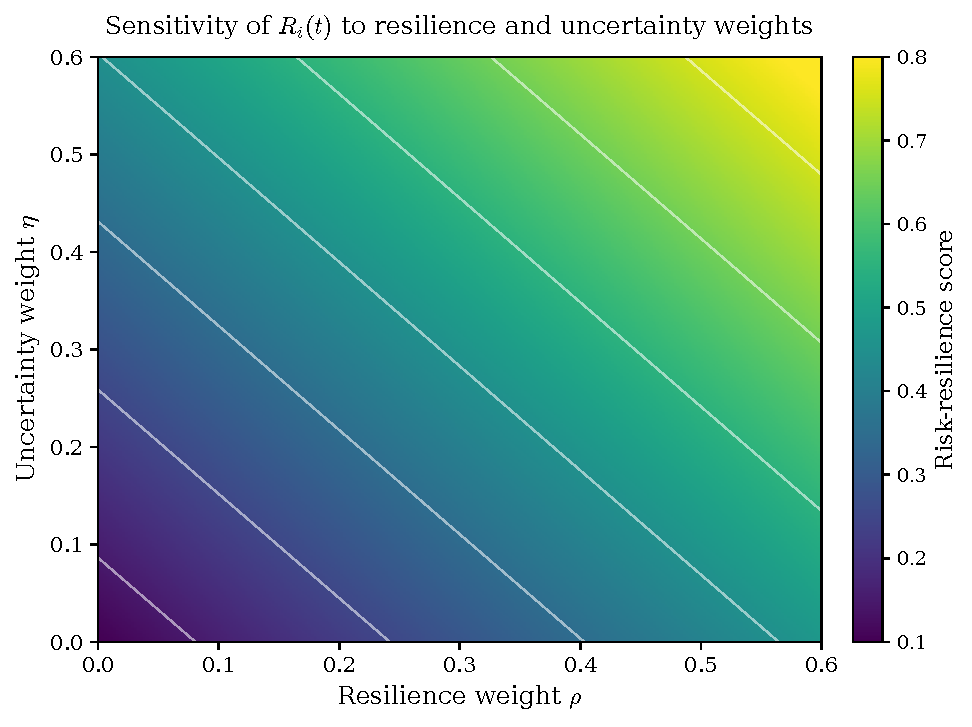
\includegraphics[width=0.70\textwidth]{fig09_lambda_eta_sensitivity.pdf}
\caption{Design-verification sensitivity of the dynamic risk--resilience index to resilience and epistemic-uncertainty weights. The plot is used as a simulation-based preference-calibration aid.}
\label{fig:weight-sensitivity}
\end{figure}

\begin{figure}[H]
\centering
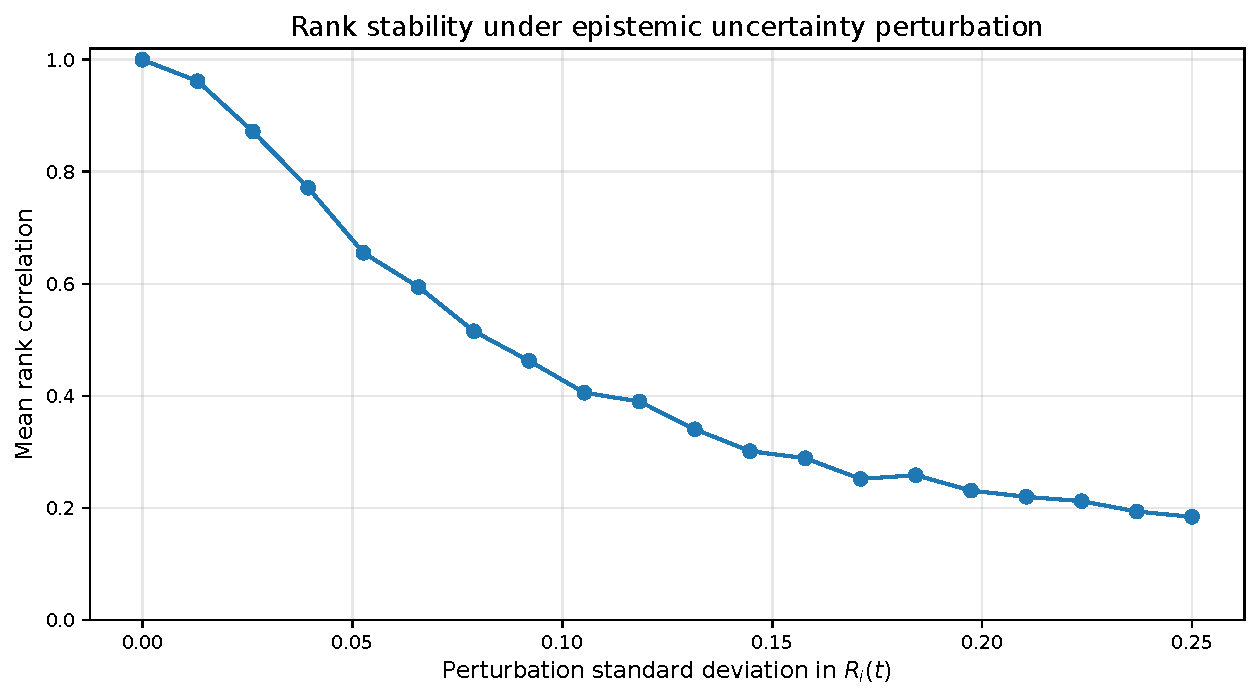
\includegraphics[width=0.70\textwidth]{fig10_rank_stability_uncertainty.pdf}
\caption{Rank-stability check under epistemic perturbation. The curve documents how maintenance rankings change as uncertainty in the input score components increases.}
\label{fig:rank-stability}
\end{figure}

High uncertainty should not automatically imply immediate repair. The VoI gate compares the expected value of inspection or monitoring against its cost \cite{thons2018,memarzadeh2016}:
\begin{equation}
\mathrm{NVI}_i(e)=\mathrm{EVSI}_i(e)-\kappa_e,\qquad e\in\{\mathrm{inspect},\mathrm{monitor}\}.
\end{equation}
An information action is selected when
\begin{equation}
\widetilde{U}_i(t)\ge u^\star
\quad \mathrm{and}\quad
\max_e \mathrm{NVI}_i(e)>0.
\end{equation}
Otherwise the asset is routed to a terminal action such as defer, repair, reinforce, or replace according to the constrained action policy.

\subsection{Graph augmentation and constrained planning}

For structurally or operationally coupled systems, a directed weighted graph $G=(\mathcal{S},\mathcal{E},W)$ is used to compute normalized centrality $\pi_i$ and cascade susceptibility $\sigma_i$ \cite{ouyang2014,newman2003}. The graph-augmented terms are
\begin{equation}
\widetilde{C}_i^G=
\frac{\widetilde{C}_i(1+\gamma\pi_i)}{1+\gamma},
\qquad
\widetilde{RTO}_i^G=
\mathrm{clip}(\widetilde{RTO}_i+\zeta_R\sigma_i,0,1).
\end{equation}
Reference-based normalization removes rank-reversal artifacts caused by rescaling scalar attributes when extreme assets are inserted or removed. Graph descriptors, however, are intrinsically topology-dependent: adding or deleting nodes and edges can change centrality $\pi_i$ and cascade susceptibility $\sigma_i$ even for retained assets. For governance-grade use, these quantities should therefore be computed on a fixed reference topology, such as the as-designed structural or operational dependency graph, or reported together with a topological perturbation sensitivity analysis.

The maintenance plan is then selected under budget, capacity, and at-most-one-action constraints. For each feasible action $a$ on asset $i$, the implementation stores relative cost, crew demand, degradation-reduction effect, uncertainty-reduction effect, and recovery-reduction effect. This allows score-order policies, greedy benefit--cost policies, random feasible-policy sampling, and NSGA-II multiobjective search to be compared under the same action set.

\subsection{Algorithmic workflow of the computational model}

The proposed model is implemented as a deterministic workflow once the stochastic inputs, random seed, and decision parameters are fixed. Table~\ref{tab:algorithm-workflow} summarizes the computational steps that map raw evidence and simulated states to a feasible action plan.

\begin{table}[H]
\centering
\scriptsize
\caption{Algorithmic workflow of the Bayesian risk--resilience computational decision model.}
\label{tab:algorithm-workflow}
\begin{tabular*}{\textwidth}{@{\extracolsep{\fill}}>{\raggedright\arraybackslash}p{0.13\textwidth}>{\raggedright\arraybackslash}p{0.28\textwidth}>{\raggedright\arraybackslash}p{0.29\textwidth}>{\raggedright\arraybackslash}p{0.21\textwidth}}
\toprule
Step & Input & Computation & Output \\
\midrule
1 & Asset attributes, class, failure mode, inspections, events & Gamma--Poisson posterior and predictive probability & $P_i^{pred}$, posterior variance \\
2 & Safety, operational, environmental, recovery descriptors & Reference-based normalization and graph adjustment & $\widetilde{C}_i^G$, $\widetilde{RTO}_i^G$ \\
3 & Data completeness, conflict, sensor and model mismatch terms & Epistemic-audit aggregation & $\widetilde{U}_i$ \\
4 & $P_i^{pred}$, $\widetilde{C}_i^G$, $\widetilde{RTO}_i^G$, $\widetilde{U}_i$ & DSMP additive value model in Eq.~\eqref{eq:score} & DSMP priority score \\
5 & Uncertainty and information cost & VoI gate for inspect/monitor routing & Information or direct-action route \\
6 & Action effects, budget, crew capacity, at-most-one-action constraint & Score-order, greedy, MCDA, random, or NSGA-II policy & Feasible action plan and Pareto candidates \\
\bottomrule
\end{tabular*}
\end{table}

\section{Simulation-Based Computational Validation Protocol}

\subsection{Synthetic degradation and limit-state simulator}

The validation experiment generates $N=300$ assets distributed across six structural classes: primary frame, secondary frame, support node, connection cluster, foundation interface, and service access. Each asset is assigned a failure mode: corrosion, fatigue, cracking, connection loss, settlement, or impact damage. A normalized degradation state evolves as
\begin{equation}
X_i(t+1)=
\mathrm{clip}\left[
X_i(t)+\delta_{c_i}+\kappa_{m_i}E_i+\phi_{m_i}L_i(t)+u_i+\varepsilon_i(t),0,1
\right],
\end{equation}
where $E_i$ is environmental exposure, $L_i(t)$ is operational load, and $u_i$ is an asset-level random effect.

The true failure event is generated through a limit-state model:
\begin{equation}
g_i(t)=R_i(t)-S_i(t),\qquad F_i(t)=\{g_i(t)\le0\},
\end{equation}
with
\begin{equation}
R_i(t)=R_{0,i}[1-X_i(t)]\exp(-\xi_i t),
\qquad
S_i(t)=S_{0,i}[1+\chi_i(t)].
\end{equation}
Monte Carlo paths provide the true failure probability used only for validation:
\begin{equation}
P_i^{true}(t,\tau)=
\frac{1}{M}\sum_{m=1}^{M}
I\left[\min_{s\in[t,t+\tau]}g_i^{(m)}(s)\le0\right].
\end{equation}
Figure~\ref{fig:limit-state} shows the limit-state interpretation used to connect the validation simulator with structural reliability language. In an applied bridge workflow, the resistance and demand variables in this representation would be informed by finite-element response, inspection measurements, material deterioration models, load histories, or digital-twin state estimates. The present experiments keep that link synthetic so that the true probability and oracle benefit are known.

\begin{figure}[H]
\centering
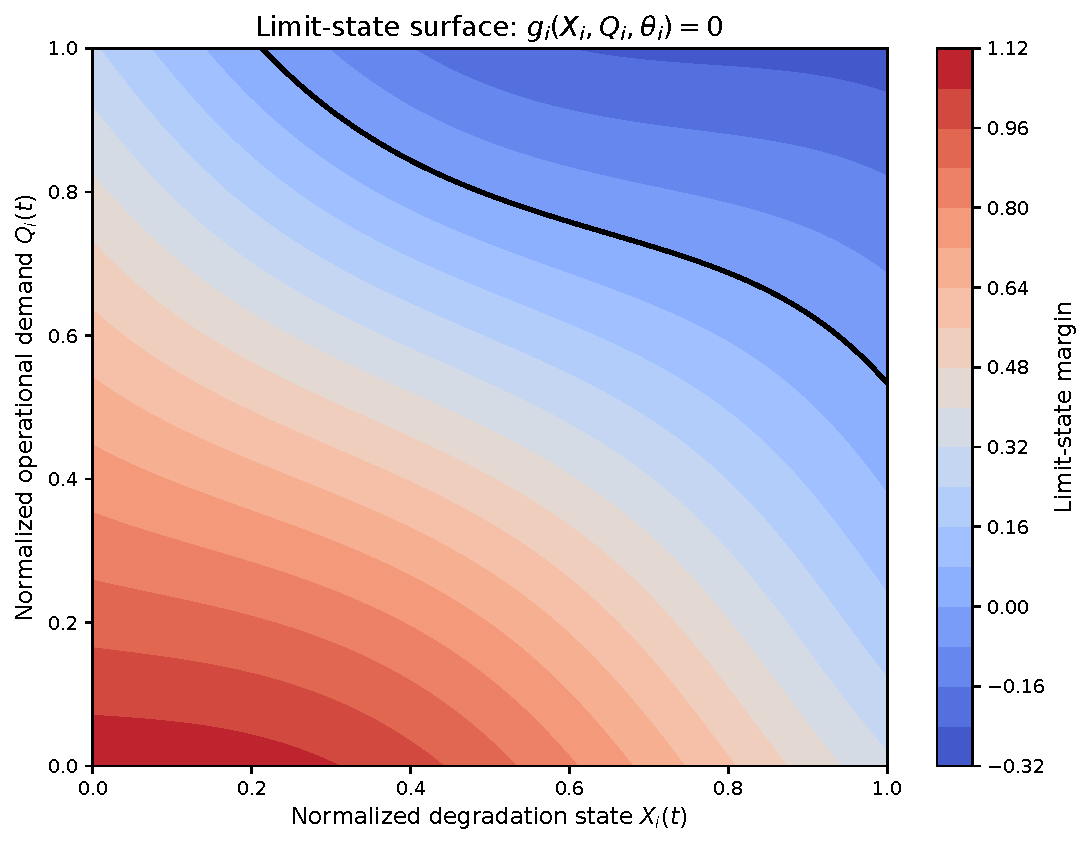
\includegraphics[width=0.66\textwidth]{fig11_limit_state_surface.pdf}
\caption{Synthetic limit-state surface used to express the validation simulator in structural reliability terms. The zero contour separates admissible and failed states.}
\label{fig:limit-state}
\end{figure}
Observed count evidence is generated separately, creating a controlled mismatch between physical failure and count-based evidence:
\begin{equation}
\lambda_i(t)=\lambda_{0,c_i}\exp(a_{m_i}X_i(t)+b_{m_i}L_i(t)+d_{m_i}E_i+u_i).
\end{equation}
This mismatch is important because it tests calibration rather than assuming the Bayesian count model is identical to the physical limit-state process.

The simulator is structured to preserve the main ingredients of a reliability-oriented maintenance problem: degradation depends on state, environment, load, class, failure mode, and asset-level heterogeneity; failure is evaluated through a resistance--demand limit state; and inspection-like count evidence is informative but imperfect. The current parameterization creates a controlled benchmark in which the true probability, true loss, and oracle policy are observable. Common shocks, spatially correlated exposure, uncertain intervention effectiveness, rare-event tails, and class-specific load histories can be represented as stress regimes of the same generator.

Table~\ref{tab:computational-experiment-flow} summarizes the input--process--output structure of the computational experiment. Table~\ref{tab:simulator-parameters} then gives the numerical parameterization used in the reported 50-seed validation protocol. The executable code contains the same values and writes them to the validation output directory.

\begin{table}[H]
\centering
\scriptsize
\caption{Input--process--output structure of the simulation-based computational validation protocol.}
\label{tab:computational-experiment-flow}
\begin{tabular*}{\textwidth}{@{\extracolsep{\fill}}>{\raggedright\arraybackslash}p{0.18\textwidth}>{\raggedright\arraybackslash}p{0.25\textwidth}>{\raggedright\arraybackslash}p{0.25\textwidth}>{\raggedright\arraybackslash}p{0.22\textwidth}}
\toprule
Block & Input & Computational process & Output \\
\midrule
Degradation & Class, failure mode, exposure, load, random effect & State update $X_i(t+1)$ & Degradation trajectory \\
Limit state & Resistance, demand, degradation path & $g_i(t)=R_i(t)-S_i(t)$ and Monte Carlo failure indicator & $P_i^{true}$, $F_i^{true}$ \\
Evidence model & Imperfect counts and exposure years & Gamma--Poisson update & $P_i^{pred}$ and uncertainty descriptors \\
Decision model & Score components, graph, budget, crew capacity & DSMP policies, baselines, VoI routing, constrained action selection & Feasible maintenance plan \\
Evaluation & Simulated truth and oracle action benefit & Calibration, regret, RRPC, downtime, ranking, rank reversal, Pareto metrics & Independent performance summaries \\
\bottomrule
\end{tabular*}
\end{table}

\begin{table}[t]
\centering
\scriptsize
\caption{Simulation and decision parameters used in the 50-seed validation protocol. The ranges summarize the class- and failure-mode-specific values implemented in the executable generator.}
\label{tab:simulator-parameters}
\begin{tabular*}{\textwidth}{@{\extracolsep{\fill}}>{\raggedright\arraybackslash}p{0.30\textwidth}>{\raggedright\arraybackslash}p{0.64\textwidth}}
\toprule
Component & Specification \\
\midrule
Portfolio and horizon & 300 assets; 10-year degradation history; 50 random seeds; 256 Monte Carlo paths per asset; budget grid $B\in\{8,12,16,20\}$; crew capacity $1.45B$. \\
Structural classes and modes & Six classes sampled with probabilities $(0.18,0.20,0.17,0.20,0.12,0.13)$ and six failure modes sampled with probabilities $(0.20,0.20,0.22,0.15,0.12,0.11)$. \\
Initial state and covariates & $X_i(0)\sim\mathrm{Beta}(2,8)$; $E_i\sim U(0,1)$; yearly $L_i(t)\sim\mathrm{Lognormal}(0,0.28)$; Monte Carlo load multiplier $\sim\mathrm{Lognormal}(0,0.30)$; $u_i\sim N(0,0.030^2)$; yearly $\varepsilon_i(t)\sim N(0,0.018^2)$. \\
Degradation parameters & Class drift $\delta_c\in[0.014,0.032]$; mode exposure coefficient $\kappa_m\in[0.008,0.020]$; mode load coefficient $\phi_m\in[0.003,0.015]$. \\
Count-evidence process & $\lambda_{0,c}\in[0.026,0.060]$; mode coefficients $a_m\in[1.05,1.55]$, $b_m\in[0.12,0.40]$, $d_m\in[0.12,0.55]$; Gamma--Poisson prior $(\alpha_0,\beta_0)=(2,4)$. \\
Limit-state variables & $R_{0,i}\sim\mathrm{Lognormal}(0,0.08)$; $S_{0,i}=R_{0,i}\,\mathrm{clip}\{N(\mu_{c_i}^{S},0.06^2),0.45,0.95\}$ with $\mu_c^S\in[0.54,0.75]$; $\xi_i\sim\mathrm{clip}\{N(0.010,0.004^2),0.001,0.030\}$; $\chi_i(t)\sim N(0,0.09^2)$. \\
Consequence and recovery & Consequence weights $(w_s,w_o,w_e)=(0.45,0.40,0.15)$; class criticality in $[0.36,0.96]$; recovery-time coefficients $r_0\in[16,56]$, $r_1\in[24,58]$, $r_2\in[7,24]$, $r_3\in[9,34]$ plus lognormal disturbance. \\
Decision weights & DSMP score weights $(\alpha,\rho,\eta)=(0.55,0.25,0.20)$; uncertainty weights $(0.40,0.35,0.25)$; data-quality weights $(0.30,0.25,0.25,0.20)$; graph coefficients $\gamma=0.40$, $\zeta=0.35$, $\zeta_R=0.35$. \\
Action effects & Defer: cost/crew/effects zero; inspect $(c,\mathrm{crew},\beta_X,\beta_U,\beta_R)=(0.05,0.25,0,0.35,0)$; monitor $(0.08,0.20,0,0.45,0)$; repair $(0.30,0.60,0.35,0.10,0.15)$; reinforce $(0.60,0.90,0.55,0.15,0.35)$; replace $(1.00,1.20,0.90,0.25,0.60)$. \\
\bottomrule
\end{tabular*}
\end{table}


\subsection{Policies and independent metrics}

The following policies are compared under the same budget and capacity levels: DSMP + VoI, DSMP direct with uncalibrated and Platt-recalibrated probabilities, a conditional-recovery DSMP variant, probability--consequence risk, severity-only ranking, consequence-only ranking, a static RCM-like rule, a VoI-only inspection rule, a greedy probability--consequence benefit--cost heuristic, and a robust TOPSIS-style MCDA baseline. Table~\ref{tab:baseline-families} groups these policies by computational role. In the results tables, ``DSMP direct'' means that the DSMP score is used to rank feasible maintenance interventions \{repair, reinforce, replace\}. ``DSMP + VoI'' uses the same evidence base and permits inspection or monitoring when the net value of information is positive. The direct policy and the VoI-gated policy therefore answer two complementary computational questions: which asset should receive an immediate intervention under resource constraints, and which asset should be routed to information acquisition because the evidence state is weak.

\begin{table}[H]
\centering
\scriptsize
\caption{Computational families represented in the policy comparison. All deployable policies use the same feasible action set, budget, and crew-capacity constraints.}
\label{tab:baseline-families}
\begin{tabular*}{\textwidth}{@{\extracolsep{\fill}}>{\raggedright\arraybackslash}p{0.22\textwidth}>{\raggedright\arraybackslash}p{0.33\textwidth}>{\raggedright\arraybackslash}p{0.36\textwidth}}
\toprule
Family & Methods & Role in the comparison \\
\midrule
Risk-based rule & Probability--consequence, severity-only, consequence-only & Classical scalar-priority references \\
Greedy optimization & Greedy probability--consequence benefit--cost & Cost-aware heuristic under the same resource constraints \\
MCDA & Robust TOPSIS & Multi-attribute decision reference using the same evidence variables \\
Maintenance logic & Static RCM-like, VoI-only inspection & Simplified industrial and information-only references \\
DSMP policies & DSMP direct, DSMP + VoI, Platt-recalibrated and uncalibrated variants & Bayesian risk--resilience decision operator and information-routing variants \\
Upper bounds and Pareto search & True-probability policies, oracle regret, NSGA-II & Non-deployable reference gap and multiobjective feasibility exploration \\
\bottomrule
\end{tabular*}
\end{table}

Two simulator-only upper-bound policies are also reported: one replaces the predicted failure probability in the DSMP score with the simulated true probability, and one ranks interventions by the true probability--consequence priority. These references quantify the performance gap caused by failure-probability mismatch. The oracle plan is computed with the ground-truth action benefit and is used only to calculate regret \cite{papakonstantinou2014a,andriotis2019,dejonge2020}.

The robust TOPSIS baseline uses the same asset information available to DSMP, but no simulated true probability. The criteria are $P_i^{pred}$, normalized consequence $C_i$, graph-adjusted recovery exposure, and normalized uncertainty. Criteria are vector-normalized, all are treated as benefit criteria for prioritization, and the TOPSIS closeness coefficient is averaged over four plausible weight vectors: $(0.40,0.30,0.20,0.10)$, $(0.30,0.35,0.25,0.10)$, $(0.30,0.25,0.25,0.20)$, and $(0.25,0.30,0.30,0.15)$. The resulting ranking is passed through the same intervention action set, budget, and capacity constraints as the direct DSMP and risk-based baselines. In addition, the multiobjective check uses the NSGA-II implementation in \texttt{pymoo} to search over discrete action assignments with objectives for residual risk, intervention cost, residual recovery exposure, and residual epistemic uncertainty \cite{deb2002,blank2020pymoo}. The reported comparisons therefore include rule-based, risk-based, MCDA, greedy benefit--cost, upper-bound, and evolutionary multiobjective references, with a shared information state that can also support MILP knapsack formulations, approximate dynamic programming, rolling-horizon policies, stochastic programming, or approximate POMDP maintenance policies \cite{debjain2014,zhangli2007,coello2004}.

The independent metrics are:
\begin{align}
\mathrm{Regret}_t &=
L^{true}(\Pi_t^{method})-L^{true}(\Pi_t^{oracle}),\\
\mathrm{RRPC}_t &=
\frac{R^{true}_{before}(t)-R^{true}_{after}(t)}
{\sum_{(i,a)\in\Pi_t^{method}}c_{i,a}+\epsilon},\\
\mathrm{Brier} &=
\frac{1}{N}\sum_{i=1}^{N}(P_i^{pred}-F_i^{true})^2,\\
\mathrm{ECE} &=
\sum_{b=1}^{B}\frac{|B_b|}{N}
\left|
\frac{1}{|B_b|}\sum_{i\in B_b}P_i^{pred}
-
\frac{1}{|B_b|}\sum_{i\in B_b}F_i^{true}
\right|.
\end{align}
Ranking quality is measured by Spearman correlation, Kendall correlation, and top-k capture against the true preventable-loss ranking. Normalization robustness is measured by pairwise rank-reversal frequency after inserting extreme assets.

The experimental unit for inferential summaries is the random seed. Monte Carlo paths are used inside each seed to estimate simulated truth; they are not treated as independent statistical replicates in the bootstrap or paired tests. Bootstrap intervals resample seed-level summaries, and Wilcoxon tests pair policies within the same seed at the reported budget level. The main table reports aggregate medians, and the same seed-level structure supports stratified calibration, ECE-bin sensitivity, and cross-portfolio train/test diagnostics when the sample size within a class or failure mode is sufficient.

\section{Computational implementation and reproducibility}

The validation layer is implemented in Python and integrated with the reproducibility pipeline. The main modules are:
\begin{itemize}[leftmargin=*]
    \item \texttt{epistemic.py}: data-quality and model-discrepancy penalties;
    \item \texttt{validation\_metrics.py}: calibration, probability recalibration, ranking, paired regret tests, bootstrap, and rank-reversal metrics;
    \item \texttt{validation\_experiments.py}: ground-truth generator, policy comparison, VoI stress test, graph perturbation, normalization stress, NSGA-II Pareto search, random Pareto reference sampling, and figure/table generation.
\end{itemize}
The consolidated project also contains the bridge/FEM data interface: nodal, bar, support, load, displacement, internal-force, stress, and reaction tables, together with the bridge generation script. These files define how structural response quantities can be moved into the decision variables of Figure~\ref{fig:decision-architecture}, providing a direct computational path from structural modeling outputs to Bayesian updating, consequence assessment, recovery estimation, and maintenance action selection.

The computational sequence is therefore:
\begin{enumerate}[leftmargin=*]
    \item ingest structural-model, inspection, monitoring, and operational evidence;
    \item update failure probability and uncertainty descriptors;
    \item compute consequence, recovery, graph, and VoI terms;
    \item solve the constrained action-selection problem;
    \item evaluate the selected policy against independent validation metrics when ground truth is available.
\end{enumerate}
The command
\begin{verbatim}
python scripts/run_all.py --seed 42 --out validation_results \
  --n-assets 300 --seeds 50 --mc-paths 256
\end{verbatim}
regenerates the validation protocol reported in this manuscript. Smaller smoke-test runs are retained only for software checks; they are not used as the primary numerical evidence.

\begin{figure}[H]
\centering
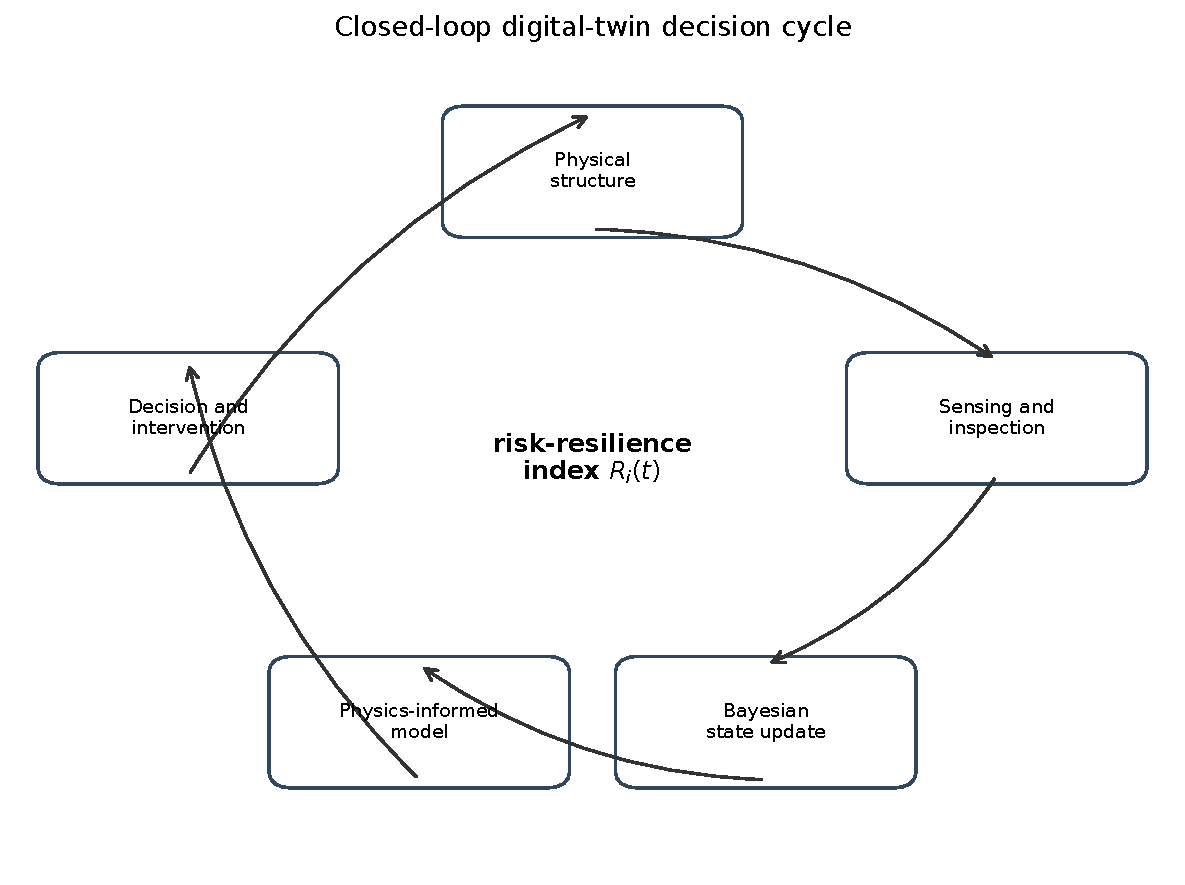
\includegraphics[width=0.78\textwidth]{fig16_digital_twin_loop.pdf}
\caption{Closed-loop positioning of the decision operator. Structural models, inspections, monitoring, and digital-twin state estimates can update the evidence base; the proposed operator acts on those inputs to prioritize information acquisition or maintenance.}
\label{fig:digital-twin-loop}
\end{figure}

\section{Results}

\subsection{Probability Recalibration and Failure-Probability Mismatch}

Figure~\ref{fig:v2-calibration} shows the calibration curves for the Gamma--Poisson predictive probability and two out-of-fold recalibration models. The raw count-based probability is strongly miscalibrated against the simulated physical truth: over 50 seeds, the median Brier score is 0.492 and the median expected calibration error (ECE) is 0.565. This is a substantive result rather than a cosmetic issue. It means that sparse event counts alone are not an adequate surrogate for the degradation and limit-state process used to generate the validation truth.

Two recalibration alternatives were tested using out-of-fold predictions. Platt recalibration maps the logit of the Gamma--Poisson predictive probability through
\begin{equation}
\mathrm{logit}\{\tilde P_i\}=a\,\mathrm{logit}\{P_i^{pred}\}+b,
\end{equation}
with $(a,b)$ fitted by penalized logistic loss. Isotonic recalibration fits a monotone nonparametric calibration curve. Recalibration is performed separately within each random seed at the asset level, not at the Monte Carlo path level. The 300 assets in a seed are randomly partitioned into five folds; for each fold, the calibrator is trained on the other four folds and evaluated only on the held-out assets. The calibration target is the simulated binary event $F_i^{true}$ sampled from the limit-state probability, not the continuous value $P_i^{true}$. The Monte Carlo paths are used to generate $P_i^{true}$ and $F_i^{true}$, but they are not treated as independent calibration samples. This cross-fitting prevents an asset's observed validation event from being used to recalibrate its own probability.

Table~\ref{tab:probability-recalibration} shows that Platt recalibration reduces the median Brier score to 0.171 and the median ECE to 0.033; isotonic recalibration also improves calibration, but is slightly less stable in this experiment. Because the simulator provides known failure events, the experiment can quantify the mismatch between a count-based predictive probability and a physical limit-state event. In applied portfolios, the same recalibration interface can use historical inspection, serviceability, intervention, or failure records, with assessment on held-out structures or time periods.

\begin{figure}[H]
\centering
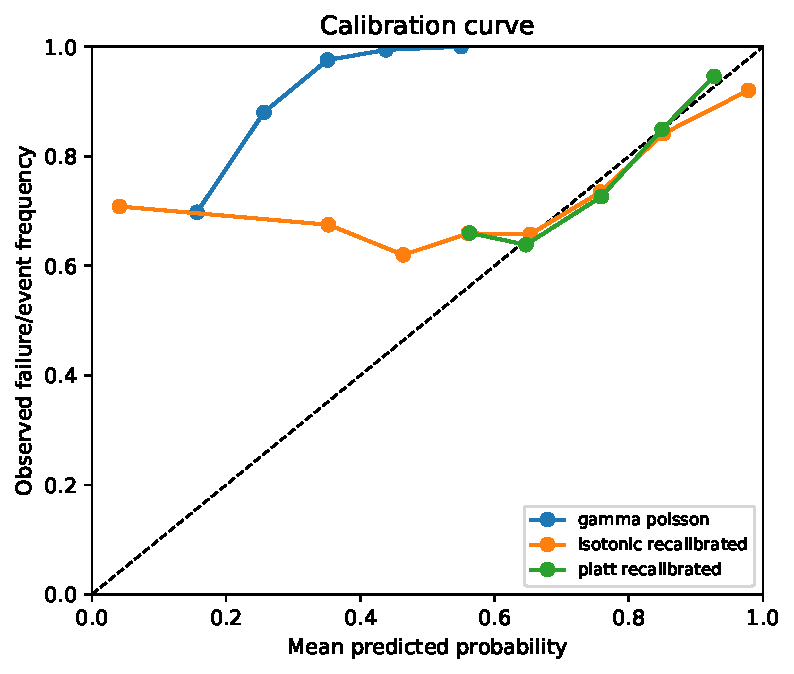
\includegraphics[width=0.72\textwidth]{figure_v2_calibration_curve.pdf}
\caption{Calibration curves comparing Gamma--Poisson predictive probabilities and out-of-fold recalibrated probabilities with simulated failure events in the ground-truth validation experiment.}
\label{fig:v2-calibration}
\end{figure}

\begin{table}[t]
\centering
\scriptsize
\caption{Out-of-fold probability recalibration results over 50 seeds. Values are medians with bootstrap 95\% intervals. Lower values are better.}
\label{tab:probability-recalibration}
\begin{tabular*}{\textwidth}{@{\extracolsep{\fill}}p{0.25\textwidth}p{0.22\textwidth}p{0.22\textwidth}p{0.22\textwidth}}
\toprule
Probability model & Brier & ECE & MSE to $P_f$ \\
\midrule
Gamma--Poisson predictive & 0.492 [0.487, 0.500] & 0.565 [0.557, 0.575] & 0.463 [0.459, 0.473] \\
Platt recalibration & 0.171 [0.168, 0.177] & 0.033 [0.030, 0.041] & 0.144 [0.141, 0.146] \\
Isotonic recalibration & 0.181 [0.174, 0.187] & 0.057 [0.047, 0.070] & 0.152 [0.149, 0.158] \\
\bottomrule
\end{tabular*}
\end{table}


\subsection{Ranking behavior}

Figure~\ref{fig:v4-ranking} summarizes top-k capture and rank correlation. The true-probability upper-bound policies rank closest to the simulated preventable-loss ordering, as expected. Among deployable policies, the DSMP scores are competitive but do not dominate every ranking statistic. The proposed framework couples ranking with constrained action selection, so a policy can improve regret even when another score has stronger top-k capture under a particular synthetic truth model.

The ranking results are therefore read as a diagnostic rather than as a single success criterion. At budget level 12, the Platt-recalibrated DSMP direct policy has stronger regret and downtime behavior than the tested deployable baselines, but its median top-k capture is 0.333. By contrast, the consequence-only ranking reaches a larger median top-k capture of 0.633 but has much higher median regret and lower downtime reduction. Static RCM has higher rank correlation than DSMP in this simulator, but its constrained action set produces substantially higher regret. These contrasts show that rank similarity to the true preventable-loss ordering and constrained maintenance value are related but not equivalent.

\begin{figure}[H]
\centering
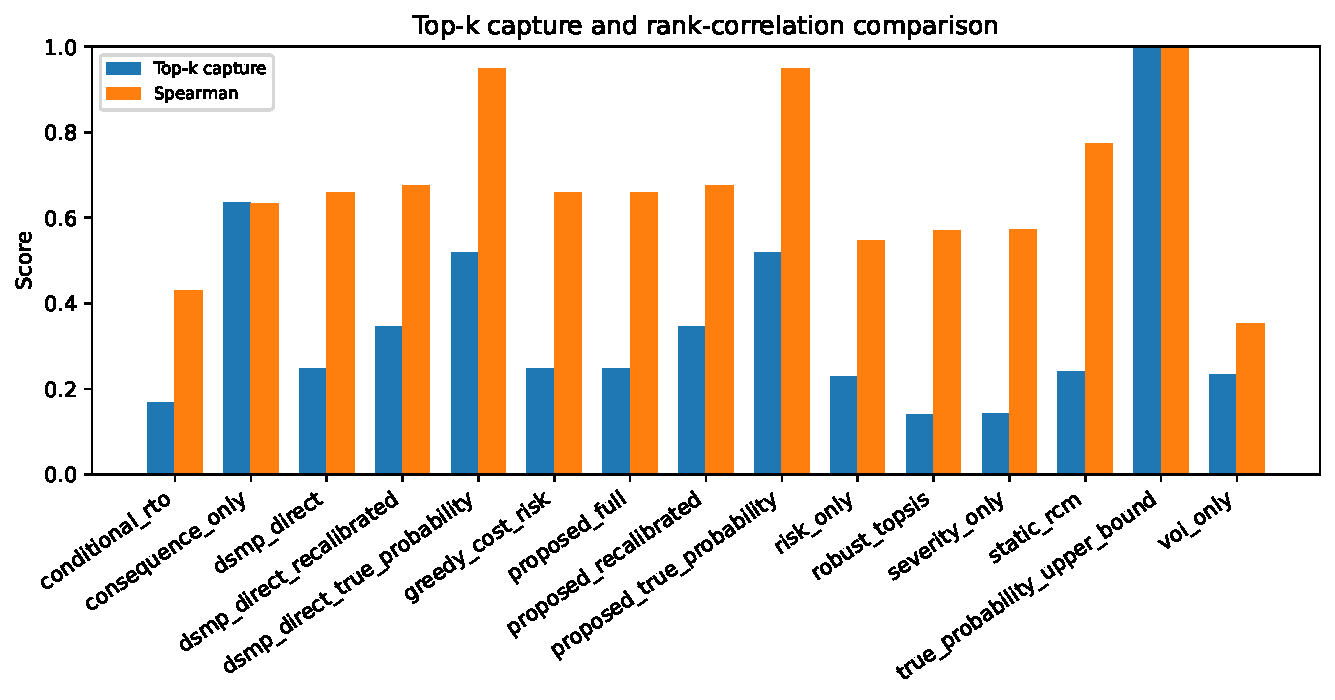
\includegraphics[width=0.82\textwidth]{figure_v4_topk_rank_comparison.pdf}
\caption{Top-k capture and rank-correlation comparison against the true preventable-loss ranking.}
\label{fig:v4-ranking}
\end{figure}

\subsection{Regret and action selection under constraints}

Table~\ref{tab:validation-main} reports the main independent metrics at budget level 12 for the 50-seed validation run. The cost-aware DSMP direct policy with Platt-recalibrated probabilities has lower median regret than the DSMP direct policy with uncalibrated probability, probability--consequence scoring, greedy probability--consequence, robust TOPSIS, and static RCM-like baselines. The improvement over the uncalibrated DSMP direct policy is modest, and its bootstrap interval overlaps zero in the paired effect table; the stronger conclusion is that recalibration substantially improves probability quality and that the Platt-recalibrated DSMP direct policy remains competitive under constrained action selection.

The DSMP + VoI rows should be interpreted separately from the direct intervention rows. With uncalibrated probabilities, DSMP + VoI remains competitive in one-step regret. With Platt-recalibrated probabilities, however, the VoI gate routes more assets toward inspection or monitoring, producing higher immediate regret and lower direct risk reduction. This behavior is consistent with its role in the present protocol: VoI makes the information-acquisition decision explicit and auditable when uncertainty is high, while direct intervention policies are the appropriate comparator for immediate one-step risk reduction.

The two true-probability rows are not deployable policies. They are included to show the remaining performance gap if the failure-probability input were replaced by the simulated physical truth. Their lower regret confirms that better structural probability models, for example from finite-element response, deterioration modeling, monitoring data, or calibrated digital twins, are likely to improve the decision layer.

\begin{table}[t]
\centering
\scriptsize
\caption{Independent validation metrics for the 50-seed ground-truth experiment (300 assets, 256 Monte Carlo paths per asset, budget level 12). Regret is reported as median [bootstrap 95\% interval]. Lower regret is better; larger RRPC and downtime reduction are better.}
\label{tab:validation-main}
\begin{tabular*}{\textwidth}{@{\extracolsep{\fill}}p{0.31\textwidth}p{0.22\textwidth}rr}
\toprule
Method & Regret [95\%] & RRPC & Downtime red. \\
\midrule
DSMP direct, Platt-recalibrated & 2.005 [1.746, 2.229] & 1.758 & 1736.8 \\
DSMP direct, uncalibrated probability & 2.191 [2.055, 2.399] & 1.736 & 1675.6 \\
DSMP + VoI, uncalibrated probability & 2.651 [2.312, 3.173] & 1.708 & 1580.7 \\
DSMP + VoI, Platt-recalibrated & 6.845 [6.578, 7.148] & 0.882 & 1167.5 \\
Greedy probability--consequence & 2.695 [2.497, 2.816] & 1.691 & 1573.2 \\
Probability--consequence score & 2.702 [2.555, 3.010] & 1.668 & 1553.7 \\
Robust TOPSIS MCDA & 3.143 [2.997, 3.288] & 1.629 & 1519.8 \\
Static RCM-like & 6.916 [6.815, 6.965] & 0.872 & 1215.4 \\
VoI-only inspection & 17.335 [17.276, 17.402] & 0.000 & 0.0 \\
\midrule
DSMP direct with true $P_f$ & 0.684 [0.591, 0.749] & 1.914 & 1908.2 \\
True-probability upper bound & 0.000 [0.000, 0.000] & 1.993 & 1972.4 \\
\bottomrule
\end{tabular*}
\end{table}


\begin{table}[t]
\centering
\scriptsize
\caption{Paired regret comparison against the DSMP direct, Platt-recalibrated policy at budget level 12. Positive effects mean the comparator has larger regret than the reference policy; negative effects indicate an upper-bound comparator with lower regret. Holm-adjusted values correct for the family of paired comparisons in this table.}
\label{tab:paired-regret-tests}
\begin{tabular*}{\textwidth}{@{\extracolsep{\fill}}>{\raggedright\arraybackslash}p{0.30\textwidth}>{\raggedright\arraybackslash}p{0.23\textwidth}rrr}
\toprule
Comparator & Median regret effect [95\%] & Pairs & Wilcoxon $p$ & Holm $p$ \\
\midrule
DSMP direct, uncalibrated probability & 0.208 [-0.151, 0.379] & 50 & 0.0305 & 0.0305 \\
DSMP + VoI, uncalibrated probability & 0.680 [0.503, 1.143] & 50 & $2.47{\times}10^{-7}$ & $7.42{\times}10^{-7}$ \\
DSMP + VoI, Platt-recalibrated & 4.804 [4.631, 5.116] & 50 & $1.78{\times}10^{-15}$ & $1.78{\times}10^{-14}$ \\
Greedy probability--consequence & 0.627 [0.520, 0.821] & 50 & $3.26{\times}10^{-7}$ & $7.42{\times}10^{-7}$ \\
Probability--consequence score & 0.669 [0.560, 0.974] & 50 & $2.64{\times}10^{-8}$ & $1.06{\times}10^{-7}$ \\
Robust TOPSIS MCDA & 1.104 [0.859, 1.301] & 50 & $1.17{\times}10^{-11}$ & $5.86{\times}10^{-11}$ \\
Static RCM-like & 4.824 [4.651, 5.143] & 50 & $1.78{\times}10^{-15}$ & $1.78{\times}10^{-14}$ \\
Consequence only & 6.494 [6.181, 7.027] & 50 & $1.78{\times}10^{-15}$ & $1.78{\times}10^{-14}$ \\
\midrule
DSMP direct with true $P_f$ & -1.272 [-1.596, -0.998] & 50 & $1.78{\times}10^{-15}$ & $1.78{\times}10^{-14}$ \\
True-probability upper bound & -2.004 [-2.229, -1.746] & 50 & $1.78{\times}10^{-15}$ & $1.78{\times}10^{-14}$ \\
\bottomrule
\end{tabular*}
\end{table}


The paired Wilcoxon comparisons in Table~\ref{tab:paired-regret-tests} are reported with Holm--Bonferroni correction. The main deployable-baseline differences remain small but statistically distinguishable after correction, except that the direct uncalibrated-probability comparison remains practically modest because the confidence interval for the median effect crosses zero. The upper-bound true-probability policies remain significantly better, which is consistent with the calibration mismatch identified above.

Figure~\ref{fig:v3-regret} shows regret as a function of budget. The Platt-recalibrated DSMP direct policy remains near the lower-regret envelope among deployable policies, while the true-probability sensitivity policies define the attainable direction when the probability model is strengthened.

The effect sizes are practically meaningful for several comparisons. Relative to the Platt-recalibrated DSMP direct policy, the median regret is about 34--35\% higher for the greedy probability--consequence and probability--consequence baselines, about 57\% higher for robust TOPSIS, and more than three times higher for severity-only and consequence-only rules. Across the tested budget grid, the Platt-recalibrated DSMP direct policy has the lowest median regret among deployable policies at budgets 8, 12, 16, and 20. Under this simulator and action model, combining Platt-recalibrated probability, consequence, recovery exposure, uncertainty audit, graph adjustment, and cost-aware action selection improves the constrained decision relative to simpler decision surfaces.

\begin{figure}[H]
\centering
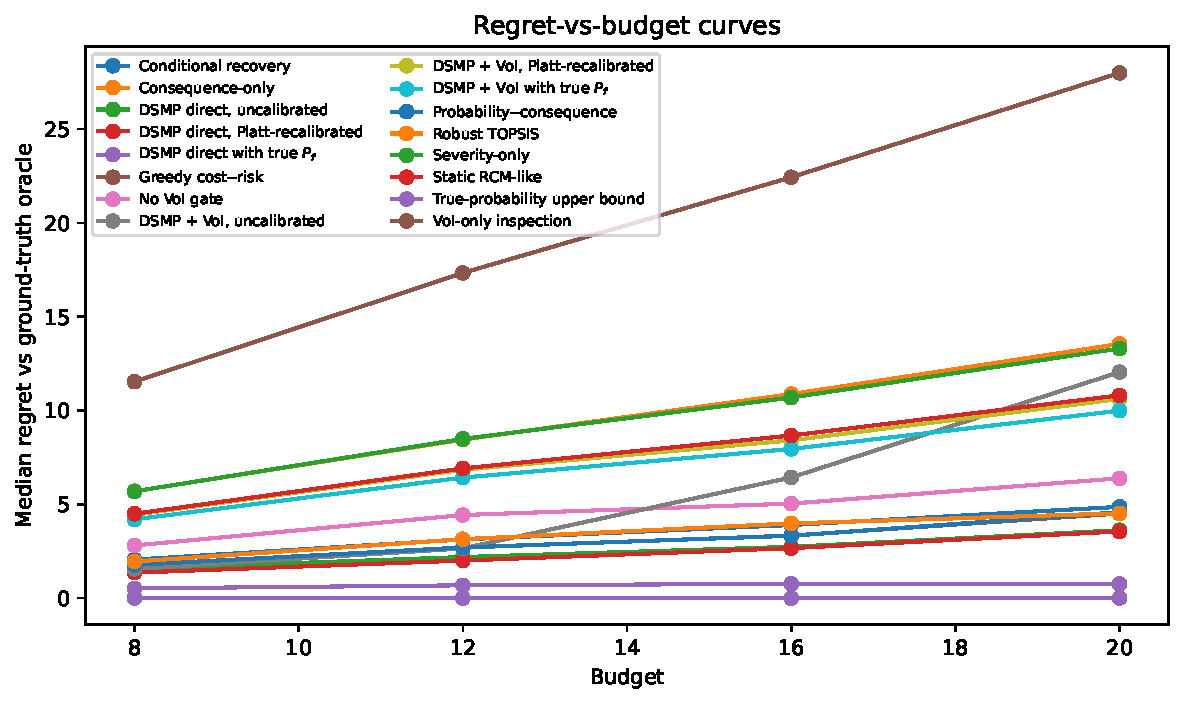
\includegraphics[width=0.82\textwidth]{figure_v3_regret_vs_budget.pdf}
\caption{Regret-vs-budget curves for the tested policies. Regret is computed against a ground-truth oracle and is not part of the proposed score.}
\label{fig:v3-regret}
\end{figure}

\subsection{VoI, ablation, and robustness}

The VoI gate is intended to route high-uncertainty assets toward inspection or monitoring only when the net value of information is positive. Figure~\ref{fig:v5-voi} maps this rule over uncertainty and information cost. The VoI-only inspection baseline has zero direct risk reduction in Table~\ref{tab:validation-main}, which is expected: information actions reduce uncertainty but do not directly reduce degradation or recovery exposure in the one-step loss model. This is why immediate-regret comparisons should distinguish direct intervention policies from information-acquisition policies.

The ablation results in Table~\ref{tab:validation-ablation} are reported as a single-seed mechanism check. They show that recovery, graph terms, probability calibration, and normalization can change the selected action set. In these experiments, the uncertainty term is most informative as an auditable representation of evidence quality and as an input to VoI routing.

\begin{figure}[H]
\centering
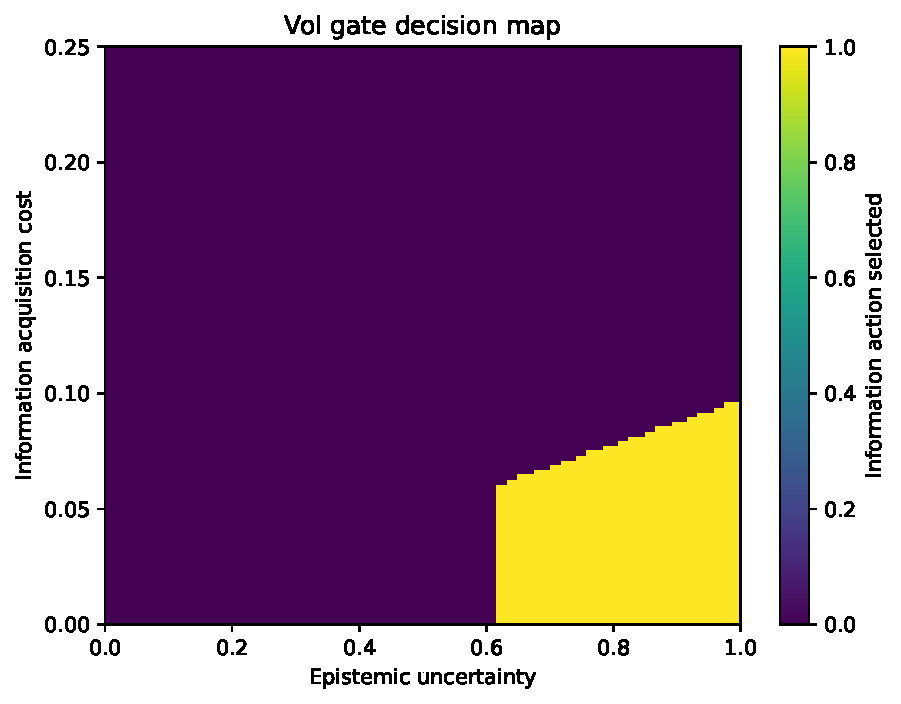
\includegraphics[width=0.70\textwidth]{figure_v5_voi_gate_decision_map.pdf}
\caption{VoI gate decision map over epistemic uncertainty and information acquisition cost.}
\label{fig:v5-voi}
\end{figure}

\begin{table}[t]
\centering
\scriptsize
\caption{Single-seed diagnostic ablation at budget level 12. This table is used to inspect mechanisms; the 50-seed results in Tables~\ref{tab:validation-main}--\ref{tab:paired-regret-tests} are the primary performance evidence.}
\label{tab:validation-ablation}
\begin{tabular*}{\textwidth}{@{\extracolsep{\fill}}p{0.35\textwidth}rrrr}
\toprule
Model variant & Regret & Risk reduction & Downtime reduction & Cost \\
\midrule
DSMP + VoI, uncalibrated probability & 2.037 & 15.299 & 1719.1 & 8.70 \\
DSMP direct, uncalibrated probability & 2.570 & 14.767 & 1661.0 & 8.70 \\
DSMP direct, Platt-recalibrated & 2.800 & 14.537 & 1609.5 & 8.70 \\
DSMP direct with true $P_f$ & 0.932 & 16.405 & 1875.0 & 8.70 \\
No recovery term & 3.322 & 14.015 & 1530.2 & 9.00 \\
No uncertainty term & 4.286 & 13.050 & 1512.5 & 11.40 \\
No VoI gate & 5.139 & 12.198 & 1390.8 & 11.40 \\
No graph augmentation & 3.863 & 13.474 & 1581.7 & 11.40 \\
Conditional RTO & 2.706 & 14.630 & 1615.9 & 9.00 \\
Portfolio min--max & 2.154 & 15.182 & 1755.5 & 9.60 \\
\bottomrule
\end{tabular*}
\end{table}


Figure~\ref{fig:v6-network} illustrates the recovery network used for graph-aware testing. The NSGA-II Pareto-feasible policies are reported in Appendix~\ref{app:pareto} as a supplementary multiobjective diagnostic, while the main comparison is carried by the calibration, regret, downtime, ranking, and robustness tables.

\begin{figure}[H]
\centering
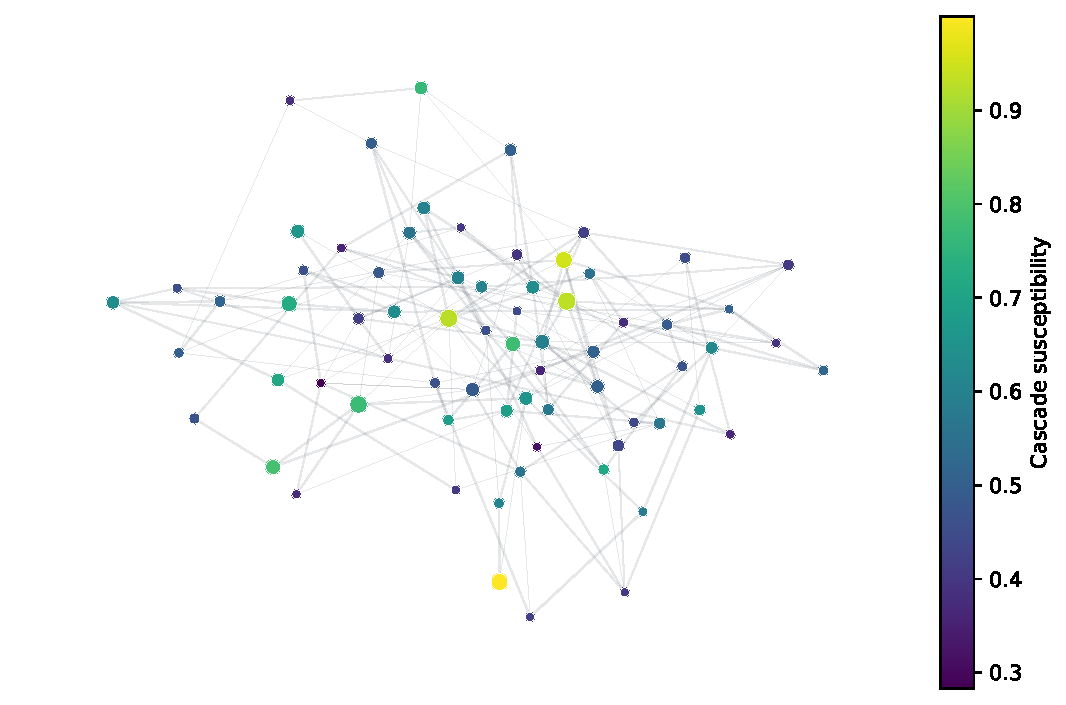
\includegraphics[width=0.78\textwidth]{figure_v6_mining_recovery_network.pdf}
\caption{Displayed recovery-network core with node size proportional to graph centrality and color indicating cascade susceptibility. Peripheral leaves are omitted for legibility.}
\label{fig:v6-network}
\end{figure}

Reference-based normalization avoided pairwise rank reversals when artificial extreme assets were inserted, while portfolio min--max normalization produced a rank-reversal frequency of 0.0676 in the representative stress sample. Figure~\ref{fig:v8-rank-reversal} and Table~\ref{tab:validation-robustness-runtime} summarize this stress test and the runtime checks. This result supports the use of fixed reference bounds when rankings must remain stable under portfolio editing.

\begin{figure}[H]
\centering
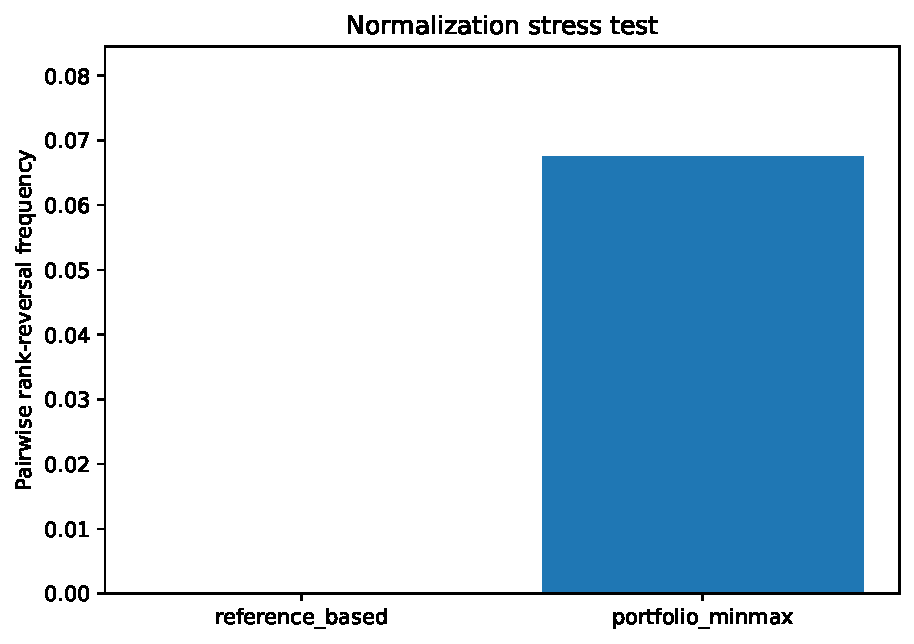
\includegraphics[width=0.66\textwidth]{figure_v8_rank_reversal_frequency.pdf}
\caption{Rank-reversal frequency under reference-based normalization and portfolio min--max normalization.}
\label{fig:v8-rank-reversal}
\end{figure}

\begin{table}[t]
\centering
\footnotesize
\caption{Normalization and computational checks for the 50-seed validation protocol.}
\label{tab:validation-robustness-runtime}
\begin{tabular*}{\textwidth}{@{\extracolsep{\fill}}llrr}
\toprule
Check & Case & Value & Auxiliary \\
\midrule
Rank reversal & reference based & 0.0000 & -- \\
Rank reversal & portfolio min--max & 0.0676 & -- \\
Runtime & DSMP + VoI & 0.009 s & 29 actions \\
Runtime & DSMP + VoI, Platt-recalibrated & 0.010 s & 13 actions \\
Runtime & DSMP direct, Platt-recalibrated & 0.017 s & 29 actions \\
Runtime & greedy probability--consequence & 0.017 s & 29 actions \\
Runtime & robust TOPSIS & 0.017 s & 29 actions \\
Runtime & oracle greedy true benefit & 0.018 s & 29 actions \\
Runtime & random Pareto search & 3.382 s & 90 nondominated solutions \\
Runtime & seeded NSGA-II Pareto search & 0.902 s & 96 nondominated solutions \\
\bottomrule
\end{tabular*}
\end{table}


\clearpage

\section{Discussion}

\subsection{Calibration, model mismatch, and constrained decision quality}

Computational structural-maintenance decision analysis benefits from rules whose inputs can be audited before an action is selected. In the proposed operator, probability, consequence, recovery, uncertainty, graph position, information value, and action cost remain separable quantities before aggregation. This provides a traceable connection between the simulated evidence streams and the final maintenance action, avoiding a single opaque condition score.

The strongest performance pattern appears when the decision layer receives calibrated failure probabilities. The uncalibrated Gamma--Poisson count model remained mismatched to the physical limit-state simulator, whereas cross-fitted Platt recalibration reduced the median Brier score from 0.492 to 0.171 and ECE from 0.565 to 0.033. With this Platt-recalibrated input, the DSMP direct policy achieved lower median regret than the deployable probability--consequence, greedy cost--risk, robust TOPSIS, and static RCM-like baselines. Policies using the simulated true failure probability still achieved lower regret, showing how strongly maintenance quality depends on the probability interface that connects evidence to the decision layer. Structural response models, inspection measurements, material deterioration models, monitoring streams, and site-specific load information can all enter through this interface.

The ranking diagnostics refine this result. The Platt-recalibrated DSMP direct policy improves regret and downtime relative to the tested deployable baselines, but it does not dominate top-k capture or all rank correlations. This distinction matters because maintenance value under finite budget and capacity is not equivalent to matching a single true ranking of preventable loss. In the present simulator, the contribution is concentrated in constrained action selection: calibrated probability, consequence, recovery exposure, uncertainty audit, graph adjustment, and cost-aware feasibility are combined into a deployable intervention rule. The probability gap exposed by the upper-bound policies is therefore a computational diagnostic: it quantifies the decision cost of model mismatch and identifies where stronger reliability or monitoring models would enter the workflow.

\subsection{Uncertainty routing, graph terms, and normalization}

The ablation study separates the roles of the individual terms. Recovery awareness is important in the tested scenario, while the uncertainty term is most useful as an audit of evidence quality and as an input to VoI routing rather than as a guaranteed regret reducer. Graph augmentation is interpretable and can affect recovery-oriented decisions, but its empirical value depends on whether the graph represents real load paths, access dependencies, or process bottlenecks. The graph terms are therefore best viewed as a structured extension whose relevance depends on the physical and operational meaning of the network.

The VoI diagnostics clarify the distinction between immediate intervention and information acquisition. Direct interventions receive immediate credit in the regret table because they reduce degradation and recovery exposure. Information actions primarily improve the evidence state, so their value is read through routing behavior, uncertainty reduction, and their interaction with recalibrated probability. The VoI-gated policy is therefore an auditable information-routing layer within the same maintenance decision architecture, while DSMP direct is the immediate intervention policy.

The strongest practical result is the normalization stress test. Portfolio-relative min--max scaling can change rankings when extreme assets are inserted or removed. Reference-based normalization avoids that artifact by fixing bounds before evaluation. For safety-related prioritization, where rankings may trigger inspection or intervention decisions, this invariance property is more than a numerical convenience; it is part of the decision audit trail \cite{kaplan1981,faber2005}.

\subsection{Multiobjective computational search and transferability}

The seeded NSGA-II search complements the regret tables by exposing feasible trade-offs among residual risk, cost, recovery exposure, and residual uncertainty. It reaches low-risk policies comparable to the best deployable rule while also identifying alternatives with lower cost, lower recovery exposure, or lower residual uncertainty. This is useful for governance because a decision maker may prefer a slightly higher residual risk if it substantially reduces cost or uncertainty exposure. Selecting a single point from the Pareto front is a preference-setting step; the computational result is the nondominated set produced under the same information, action, budget, and crew constraints.

The numerical evidence is simulation-based and addresses mathematical consistency, reproducibility, calibration, model mismatch, constrained regret, normalization stability, and multiobjective feasibility under controlled assumptions. The same decision layer can be paired with bridge, dam, offshore, lifeline, or industrial-structure records containing observed deterioration, interventions, serviceability exceedances, failures, and recovery outcomes \cite{saaty2008,brans1985,thons2018}. This modularity is the main reason for positioning the paper as a computational modeling contribution for engineering decision support.

\section{Conclusions}

This paper presented the DSMP model, a simulation-based Bayesian computational decision model for structural maintenance prioritization under epistemic uncertainty. The formulation extends probability--consequence risk by adding recovery-time exposure and auditable uncertainty terms while retaining the classical risk expression as a limiting case. The operator is connected to VoI-based information routing, graph-aware recovery/consequence adjustment, constrained maintenance planning, probability recalibration, and NSGA-II multiobjective feasibility analysis.

The validation protocol evaluates the method against a synthetic ground truth rather than against the score's own components. In the 50-seed validation run, the uncalibrated Gamma--Poisson probability was poorly calibrated, but cross-fitted Platt recalibration substantially improved Brier score and ECE. At the selected budget level, the cost-aware DSMP direct policy with Platt-recalibrated probabilities achieved lower median regret than the deployable probability--consequence, greedy cost--risk, robust TOPSIS, and static RCM-like baselines, while policies using the simulated true failure probability remained better. The ranking and VoI diagnostics show where the benefit is concentrated: constrained direct intervention improves regret under the one-step budgeted action model, and the VoI gate preserves an explicit route for information acquisition when the evidence state is weak. Reference-based normalization avoided rank reversals under portfolio stress, and seeded NSGA-II documented a feasible multiobjective trade-off front.

The resulting workflow is modular: probability models, structural response outputs, monitoring evidence, consequence descriptors, recovery estimates, action effects, and resource constraints enter through explicit computational interfaces. This structure makes the method useful as a reproducible decision-support layer for reliability-informed structural maintenance and as a benchmark for comparing alternative calibration, optimization, and multiobjective planning strategies under equal information and constraint sets.

\appendixstart
\appendix
\renewcommand{\theHequation}{A.\arabic{equation}}
\section[\appendixname~\thesection]{Supplementary Pareto Feasibility Check}
\label{app:pareto}

The validation code uses NSGA-II through \texttt{pymoo} to search feasible policies and identify nondominated plans over residual risk, cost, recovery exposure, and residual uncertainty. A random feasible-policy search is retained as a runtime and reproducibility reference. For a feasible maintenance plan $\Pi$, the Pareto check considers the objective vector
\begin{equation}
\min_{\Pi}
\left(
R_{\mathrm{res}}(\Pi),\ C(\Pi),\ RTO_{\mathrm{res}}(\Pi),\ U_{\mathrm{res}}(\Pi)
\right),
\end{equation}
where the four components denote residual risk, intervention cost, residual recovery exposure, and residual epistemic uncertainty. The decision vector assigns one of six actions to each asset: defer, inspect, monitor, repair, reinforce, or replace. Feasibility is enforced by total budget, crew-capacity, and at-most-one-action-per-asset constraints. The NSGA-II population is seeded with feasible no-action and deployable policy plans, then evolved to explore additional trade-off combinations. In the reported 300-asset instance, NSGA-II returned 96 feasible nondominated policies over this objective space. Figure~\ref{fig:v7-pareto} documents the evolutionary search layer used in the reproducible multiobjective protocol and provides a reference set for exact, approximate, or alternative evolutionary solvers under the same information and constraints.

\begin{figure}[H]
\centering
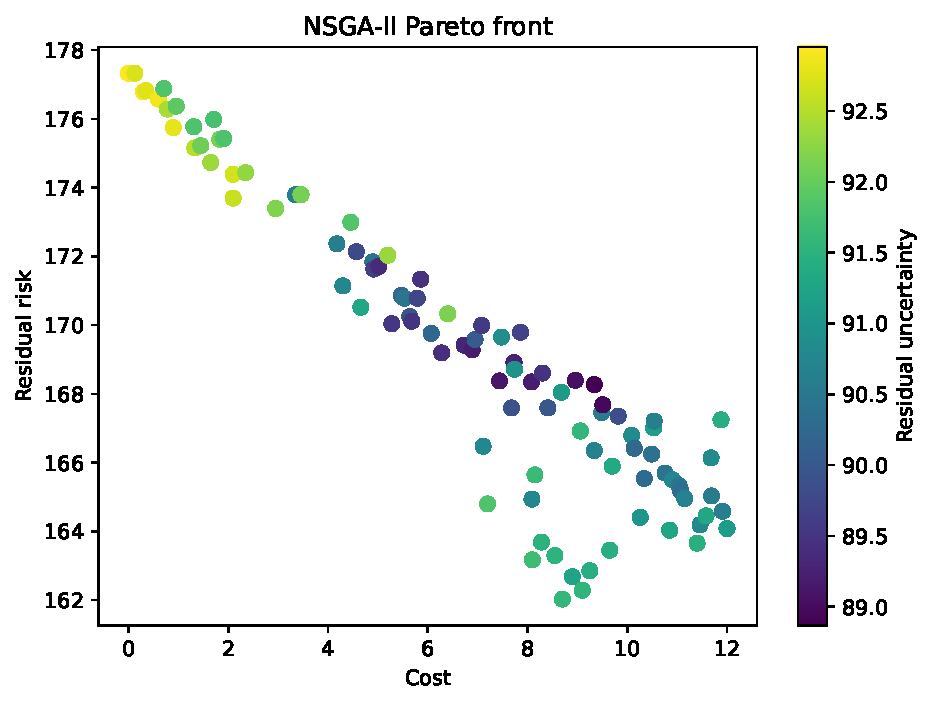
\includegraphics[width=0.70\textwidth]{figure_v7_pareto_front.pdf}
\caption{Supplementary NSGA-II Pareto-feasible policies for residual risk, cost, recovery exposure, and residual uncertainty.}
\label{fig:v7-pareto}
\end{figure}

\acknowledgement{The authors acknowledge the role of reproducible computational experiments in making reliability-based maintenance decision models transparent, testable, and reusable.}

\funding{The author(s) received no specific funding for this study.}

\authorcontributions{Conceptualization, Luis Rojas-Valdivia and Jose Garcia; methodology, Luis Rojas-Valdivia and Jose Garcia; software, Luis Rojas-Valdivia; validation, Luis Rojas-Valdivia and Jose Garcia; formal analysis, Luis Rojas-Valdivia; investigation, Luis Rojas-Valdivia; resources, Luis Rojas-Valdivia and Jose Garcia; data curation, Luis Rojas-Valdivia; writing--original draft preparation, Luis Rojas-Valdivia; writing--review and editing, Luis Rojas-Valdivia and Jose Garcia; visualization, Luis Rojas-Valdivia; supervision, Jose Garcia. All authors reviewed and approved the final version of the manuscript.}

\availabilityofdataandmaterials{The computational workflow is provided as executable Python code in the accompanying repository. The validation run reported in this manuscript writes processed data, figures, and tables under \texttt{validation\_results\_50x256/}. The full protocol can be regenerated with \texttt{scripts/run\_all.py}. All datasets used in this manuscript version are simulated validation datasets generated by the executable protocol.}

\ethicsapproval{Not applicable.}

\conflictsofinterest{The authors declare no conflicts of interest.}

\abbreviations{Abbreviations}{
\noindent
\begin{tabular}{@{}ll}
DSMP & Dynamic Structural Maintenance Prioritization\\
ECE & Expected calibration error\\
NSGA-II & Non-dominated sorting genetic algorithm II\\
RCM & Reliability-centered maintenance\\
RRPC & Risk reduction per cost\\
TOPSIS & Technique for order preference by similarity to ideal solution\\
VoI & Value of information
\end{tabular}}

\reftitle{References}
\bibliography{references}

\end{document}
